\section{MC studies}
\label{sec:mc_study}
\subsection{Simulation setup}
The expected number of neutrino events in the water-in Wagasci detector
is predicted by Monte Carlo simulations.
Neutrino beam flux at the detector location is simulated by T2K neutrino flux generator, JNUBEAM. Neutrino interactions with target materials are simulated by a neutrino interaction simulator, NEUT. Detector responses are simulated using GEANT4-based simulation.


The detector geometry in the simulation so far is different from the actual setup as shown in Figure \ref{fig:wagasci_mc_geometry}.
The active neutrino target region consists of four WAGASCI modules.
The size of the WAGASCI module is same as the actual one: 1000 mm $\times$ 1000 mm in the x and y directions and 500 mm along the beam direction (z-direction).
%An event display of a MC event in the WAGASCI detectors is shown in Figure \ref{fig:wagasci_event_display}.
Two Side-MRD modules are installed either side of the Wagasci modules.
Each Side-MRD module consists of ten iron plates whose dimension is 30 mm (thickness) $\times$ 2000 mm (height) $\times$ 3200 mm (width). 
The distance between the Side-MRD modules and WAGASCI modules is 800 mm.
The downstream-MRD is equivalent to the Baby-MIND, but without the magnetic field.
It consists of thirty iron plates whose dimension is  30 mm (thickness) $\times$ 2000 mm (height) $\times$ 4000 mm (width).
The distance between the downstream-MRD modules and WAGASCI modules is 800 mm.
Update of the study with the actual geometry is now underway.

\begin{figure}[tbhp]
\begin{center}
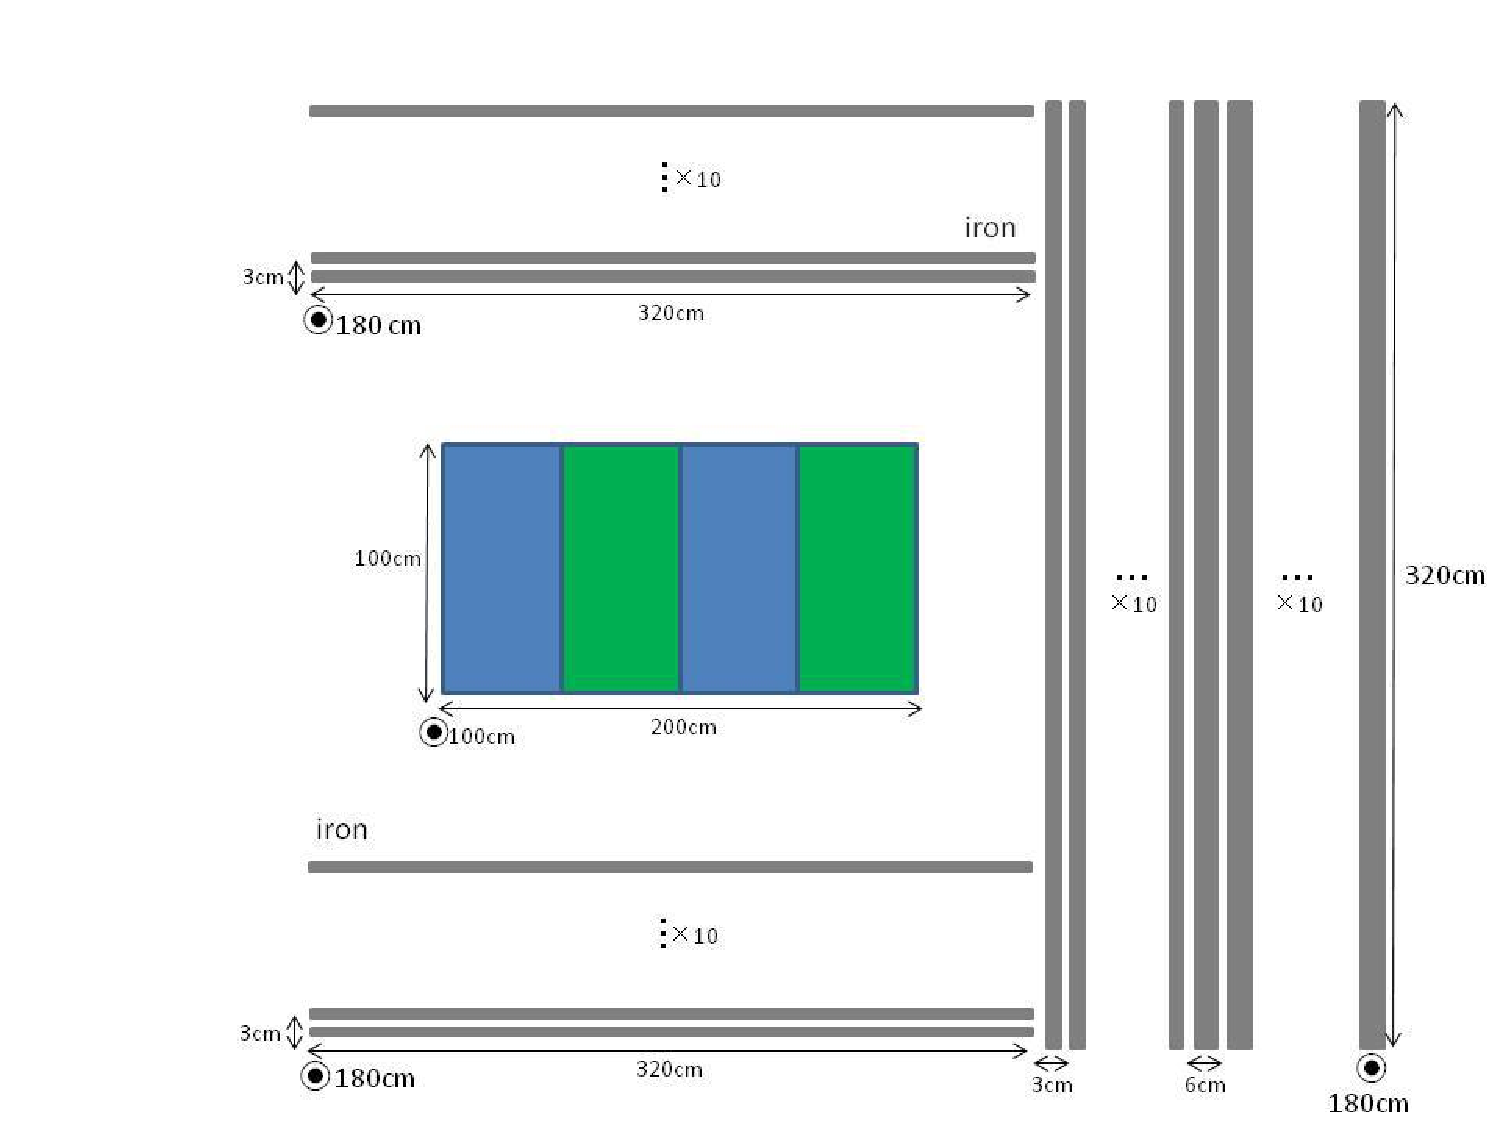
\includegraphics[width=0.8\linewidth]{fig/wagasci_mc_geometry.pdf}
% \includegraphics[width=0.8\linewidth]{fig/all_detector2.pdf}
\end{center}
\caption{
Geometry of the detectors in the Monte Carlo simulation.}
\label{fig:wagasci_mc_geometry}
\end{figure}

%\begin{figure}[tbh]
%\begin{center}
%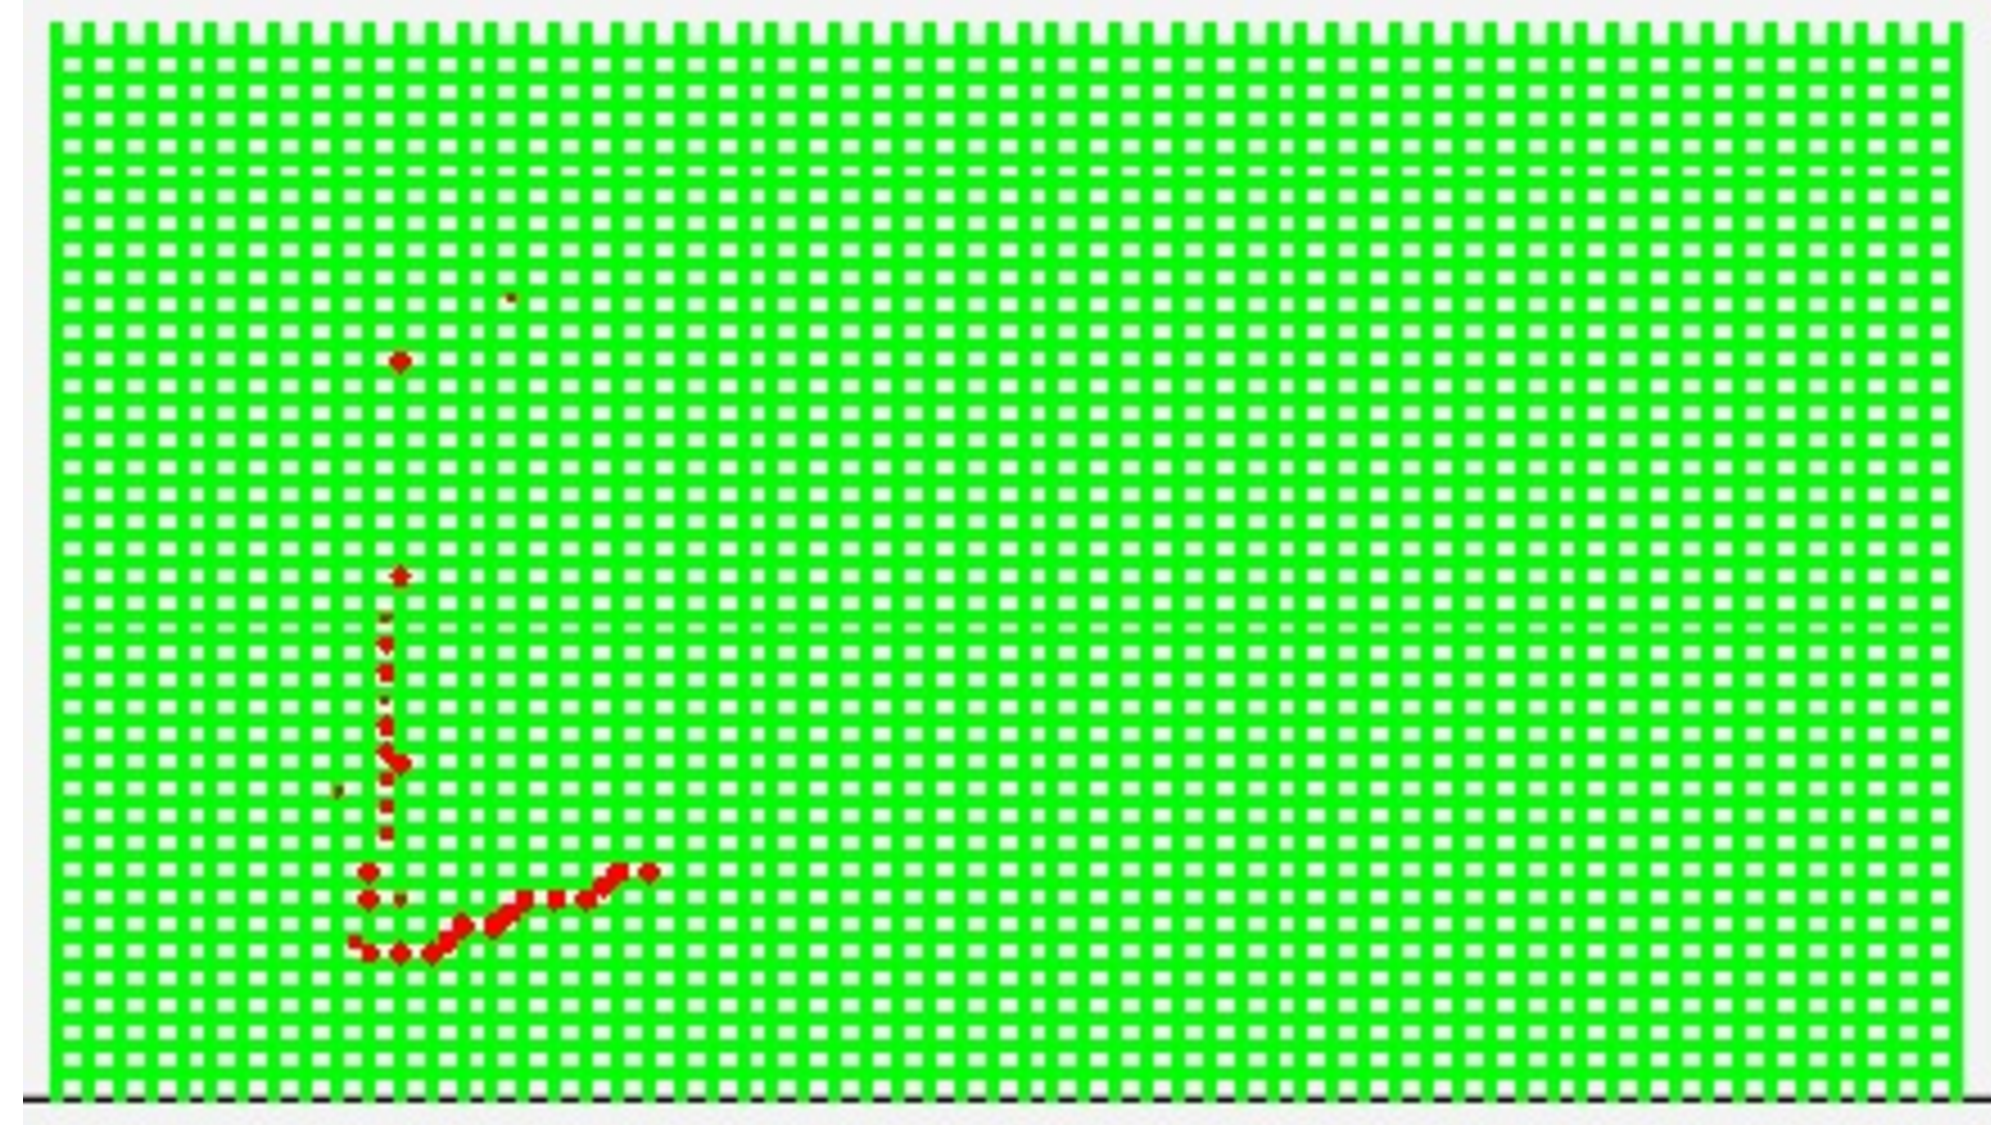
\includegraphics[width=0.8\linewidth]{fig/wagasci_event_display.pdf}
%% \includegraphics[width=0.8\linewidth]{fig/all_detector2.pdf}
%\end{center}
%\caption{
%An event display of MC event in WAGASCI detectors. Green lines are scintillators and red circles are the hit channels.}
%\label{fig:wagasci_mc_geometry}
%\end{figure}

% In order to estimate backgrounds from neutrino interactions in the wall and floor of the experimental hall, the geometry of the experimental hall is implemented in the GEANT4-based detector simulation.

To simulate the signal, the energy deposit inside the scintillator is converted into the number of photons. 
The effects of collection and attenuation of the light in the scintillator and the WLS fiber are simulated, and the MPPC response is also taken into account. 
The light yield is smeared according to statistical fluctuations and electrical noise.


\subsection{Event selection}

Tracks are reconstructed in two-dimensional planes in each sub-detector.
Then, track matching among the sub-detectors and three-dimensional track reconstruction are performed.
These analysis tools have been developed from the software tools by the T2K INGRID and in mature stage already.

The events are selected as follows.
The starting point of the track is required to be 50~mm away from the edge of the WAGASCI module. This is to remove the background from the outside.
% as shown in Fig. \ref{fig:fv_cut}.
% \begin{figure}[tbh]
% \begin{center}
%   \begin{subfigure}{0.48\textwidth}
%     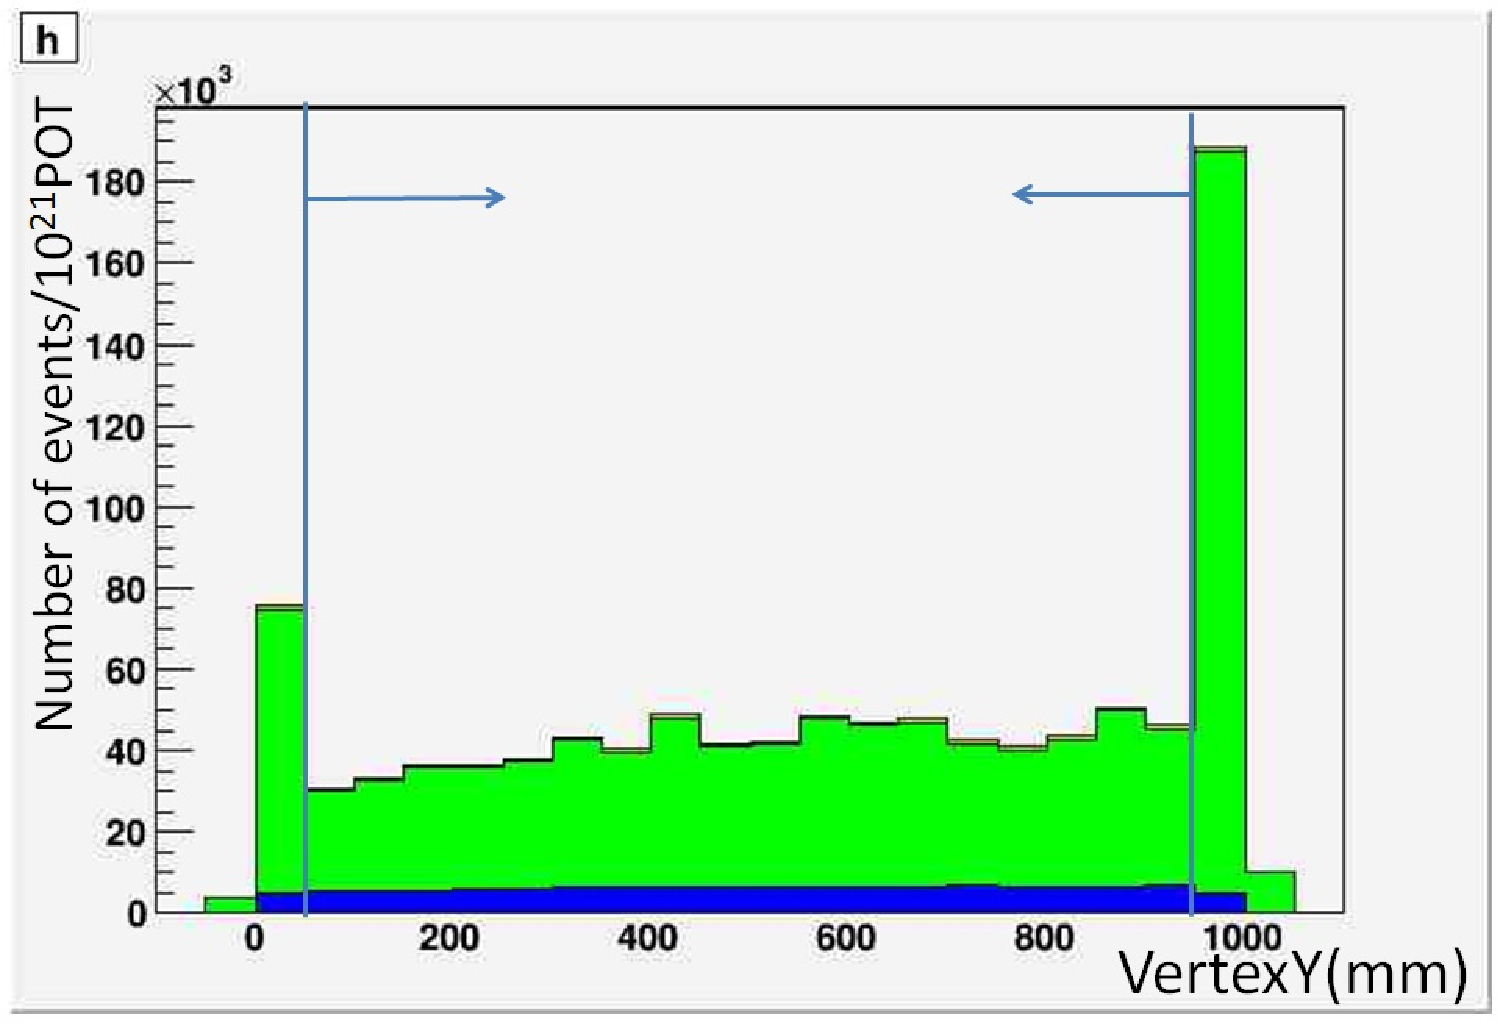
\includegraphics[width=\linewidth]{fig/fv_cut_y.pdf}
%    \end{subfigure}
%  \begin{subfigure}{0.48\textwidth}
%      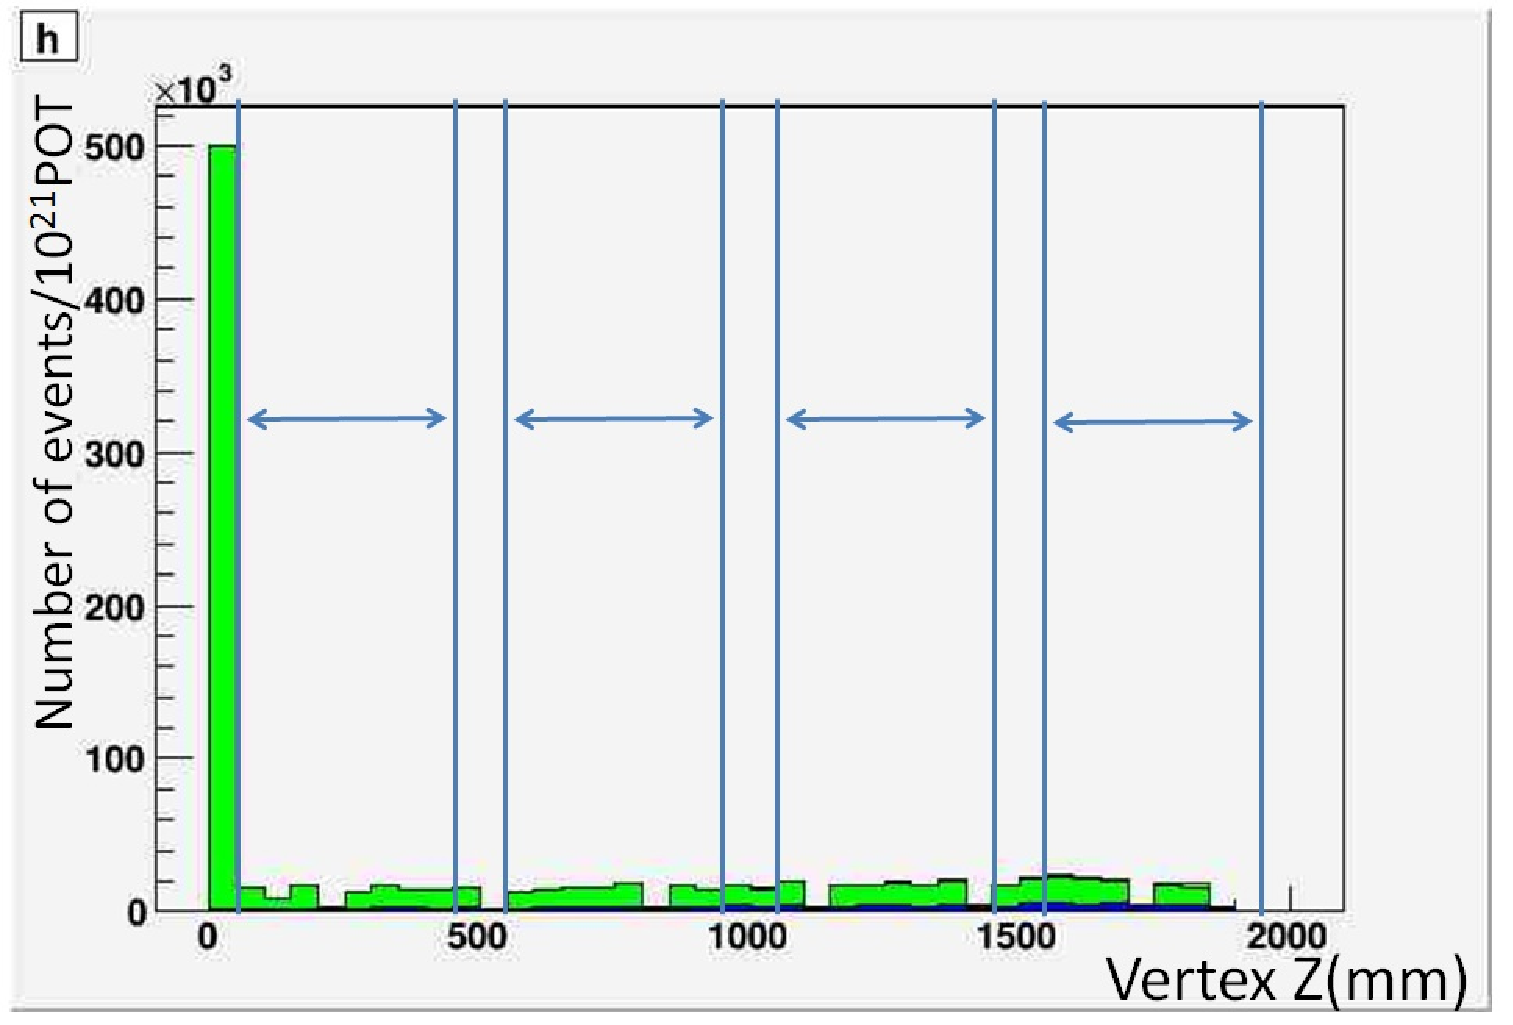
\includegraphics[width=\linewidth]{fig/fv_cut_z.pdf}
%    \end{subfigure}    
%    \end{center}
%  \caption{Event selection with the vertex of the track.
% Blue hist. are events from the WAGASCI modules, green hist. are events from the experimental hall, % and yellow hist. are events from the Side-MRD modules and the downstream-MRD.
% }
% \label{fig:fv_cut}
% \end{figure}
The longest track has to penetrate more than one (five) iron plates in Side-MRD modules (Baby-MIND).
This cut select a muon track and rejects backgrounds from NC and neutral particles.
%as shown in Figure \ref{fig:penetrated_iron_plates_cut}.
Then, in order to determine the muon momentum, it is required that the longest track stops in MRDs (Side-MRD modules and Baby-MIND) or penetrate all iron plates.
% \begin{figure}[tbh]
%  \begin{center}
%   \begin{subfigure}{0.48\textwidth}
%      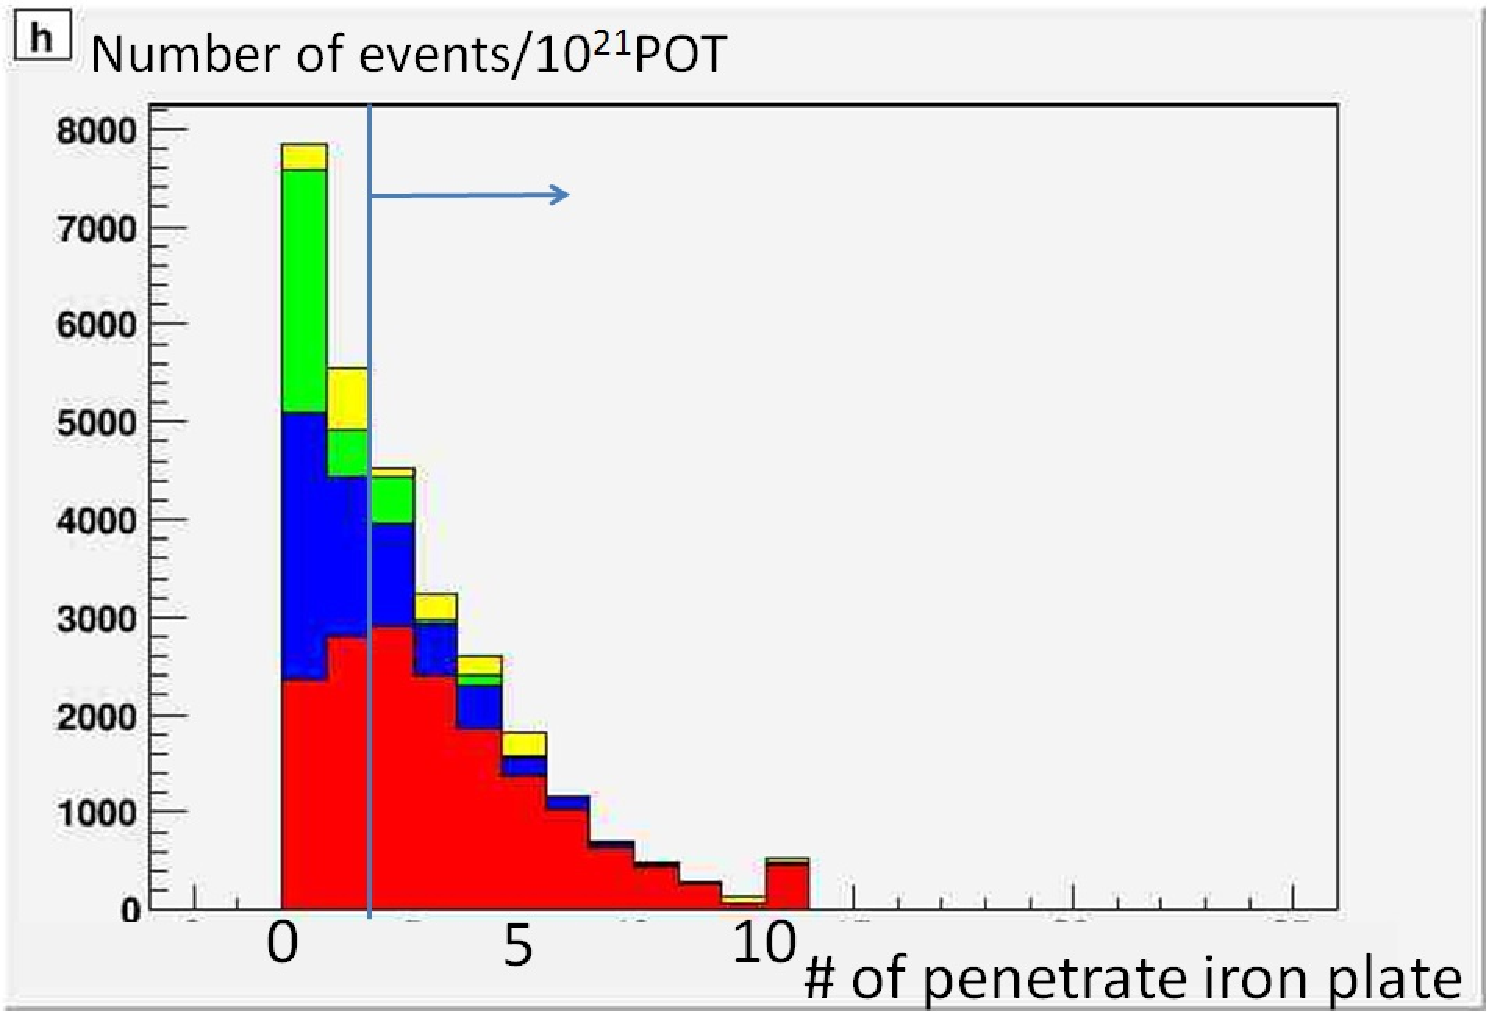
\includegraphics[width=\linewidth]{fig/penetrated_iron_plates_cut_sidemrd.pdf}
%     \end{subfigure}
%   \begin{subfigure}{0.48\textwidth}
%     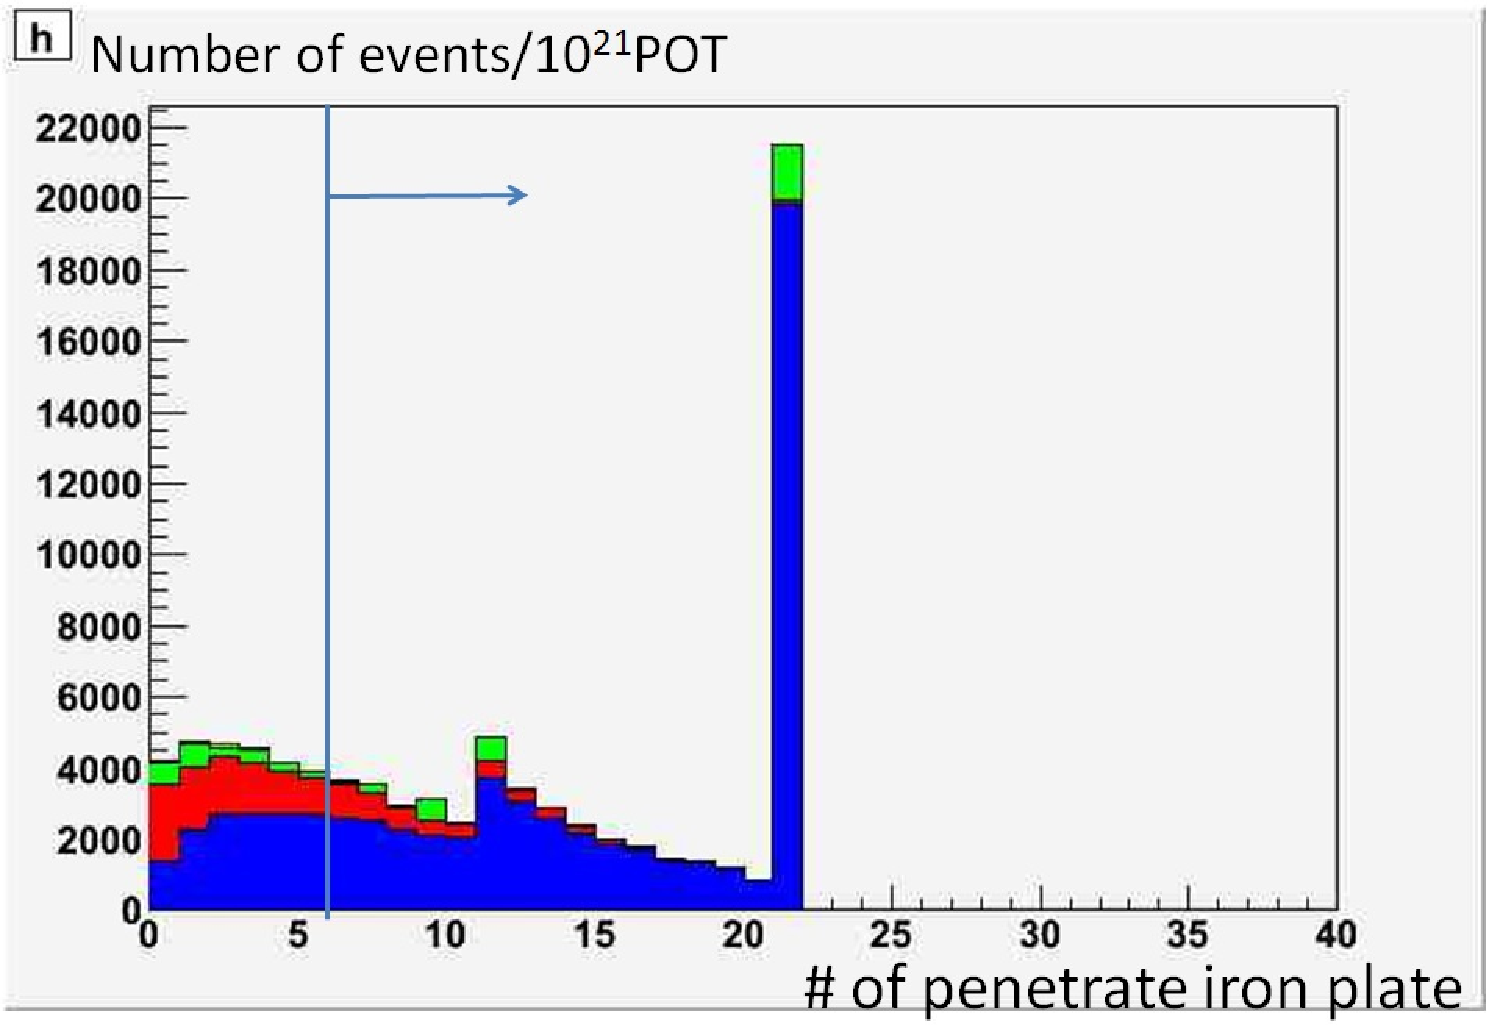
\includegraphics[width=\linewidth]{fig/penetrated_iron_plates_cut_babymind.pdf}
%     \end{subfigure}    
%     \end{center}
%   \caption{
% Event selection with the number of the penetrated iron plates in the side-MRD modules (left) and the Baby-MIIND (right).
% Blue and red hist. are events from the WAGASCI modules, green hist. are events from the experimental hall, and yellow hist. are events from the Side-MRD modules and the Baby-MIND.
% }
% \label{fig:penetrated_iron_plates_cut}
% \end{figure}

% \subsection{Selected events}


Table~\ref{tab:expected_num_events}  shows numbers of the selected events in one water-in WAGASCI module after the event selection.
We expect 4,239 (1,666) events from charged-current interaction on $\mathrm{H_2O}$ with $5 \times 10^{20}$  POT in (anti)neutrino-mode with one water-in WAGASCI module.
The purity, when interactions on CH is counted as background, is 78\% for the neutrino-mode.
There is a significant contamination from the wrong-sign (neutrino) interaction for antineutrino-mode, however, we expect that
it will be removed with efficiency higher than 90\% by Baby MIND.
%\begin{table}[htb]
%  \begin{center}
%    \caption{Expected number of the neutrino-candidate events in one water-in WAGASCI module with 1$\times 10^{21}$ POT in neutrino-mode.}
%    \begin{tabular}{c|ccc|c} \hline
%Cut   & CC & NC & Scinti Bkg. & Total \\ \hline
%Reconstructed & 18093.2 & 699.7 & 4698.3 & 23491.2 \\
%FV & 15150.8 & 588.4 & 3934.8 & 19673.9 \\
%Pene. iron & 11264.3 & 237.3 & 2875.4 & 14377.0 \\
%Stop/Penetrate MRDs & 8478.2 & 214.0 & 2173.1 & 10865.2 \\ \hline
%after all cuts & 78.0 \% & 2.0 \% & 20.0 \% & 100 \% \\
%\hline
%    \end{tabular}
%    \label{tab:expected_num_events_neutrino_beam}
%  \end{center}
%\end{table}
%\begin{table}[htb]
%  \begin{center}
%    \caption{Expected number of the antineutrino-candidate events in one water-in WAGASCI module with 1$\times 10^{21}$ POT in antineutrino-mode.}
%    \begin{tabular}{c|cccc|c} \hline
% Cut   & CC & NC & Scinti Bkg. & Wrong sign bkg & Total \\ \hline
%Reconstructed & 6499.7 & 107.3 & 2234.4 & 2330.8 & 11172.1 \\ 
%FV & 5457.9 & 89.3 & 1873.5 & 1946.6 & 9367.1 \\ 
%Pene. iron & 4172.3 & 30.8 & 1440.9 & 1560.6 & 7204.6 \\ 
%Stop/Penetrate MRDs & 3331.5 & 28.5 & 1120.3 & 1121.2 & 5601.5 \\ \hline
%after all cuts & 59.5 \% & 0.5 \% & 20.0 \% &  20.0 \% & 100 \% \\
%\hline
%    \end{tabular}
%    \label{tab:expected_num_events_antineutrino_beam}
%  \end{center}
%\end{table}
\begin{table}[htbp]
  \begin{center}
    \caption{Expected number of the selected neutrino-candidate events in one water-in WAGASCI module with $5\times 10^{20}$ POT in each of neutrino-mode and antineutrino-mode.
      Note that the wrong sign component will be reduced by one order by applying the charge selection by Baby MIND.}
    \begin{tabular}{ccccc} \hline
   & CC on $\mathrm{H_2O}$ & NC on $\mathrm{H_2O}$ & Interaction on CH  & wrong sign interaction\\ \hline
   $\nu$-mode & 4239 & 107 & 1087 & (negligible) \\ \hline
   anti-$\nu$-mode & 1666 & 14 & 560 & (561) \\
\hline
    \end{tabular}
    \label{tab:expected_num_events}
  \end{center}
\end{table}


Table \ref{tab:expected_num_cc_events} and \ref{tab:expected_num_ccfsi_events} summarize
contributions classified by the interaction types and final state topologies for the selected charged current-interaction events, respectively.
%
\begin{table}[htbp]
  \begin{center}
    \caption{Interaction types for the selected charged-current events.}
    \begin{tabular}{c|cccc} \hline
& CCQE & 2p2h & CC resonant $\pi$  & CC-DIS \\ \hline
$\nu$-mode & 48.4 \% & 9.7 \% & 27.1 \% & 14.7 \% \\
anti-$\nu$-mode &  57.1 \% & 8.2 \% & 17.3 \% & 17.3 \% \\
\hline
    \end{tabular}
    \label{tab:expected_num_cc_events}
  \end{center}
\end{table}
%
\begin{table}[htbp]
  \begin{center}
    \caption{Final state topologies for the selected charged-current events.}
    \begin{tabular}{c|cccc} \hline
& CC0$\pi$ & CC1$\pi$ & CC2$\pi$ & CCn$\pi$ \\ \hline
      $\nu$-mode & 67.4 \% & 20.9 \% & 3.0 \% & 8.7 \% \\ \hline
      anti-$\nu$-mode & 79.5 \% & 16.3 \% & 1.2 \% & 3.0 \% \\\hline
    \end{tabular}
    \label{tab:expected_num_ccfsi_events}
  \end{center}
\end{table}

Figure \ref{fig:angle_allcut} shows the reconstructed angles of the longest tracks in the selected events in the neutrino-mode and the anti-neutrino mode.
Figure \ref{fig:endpoint_longest_track} shows the iron plane numbers in Side-MRD and Baby-MIND corresponding to the end points of the longest tracks in the selected events in the neutrino-mode and the anti-neutrino mode.
%
\begin{figure}[tbh]
 \begin{center}
  \begin{subfigure}{0.48\textwidth}
     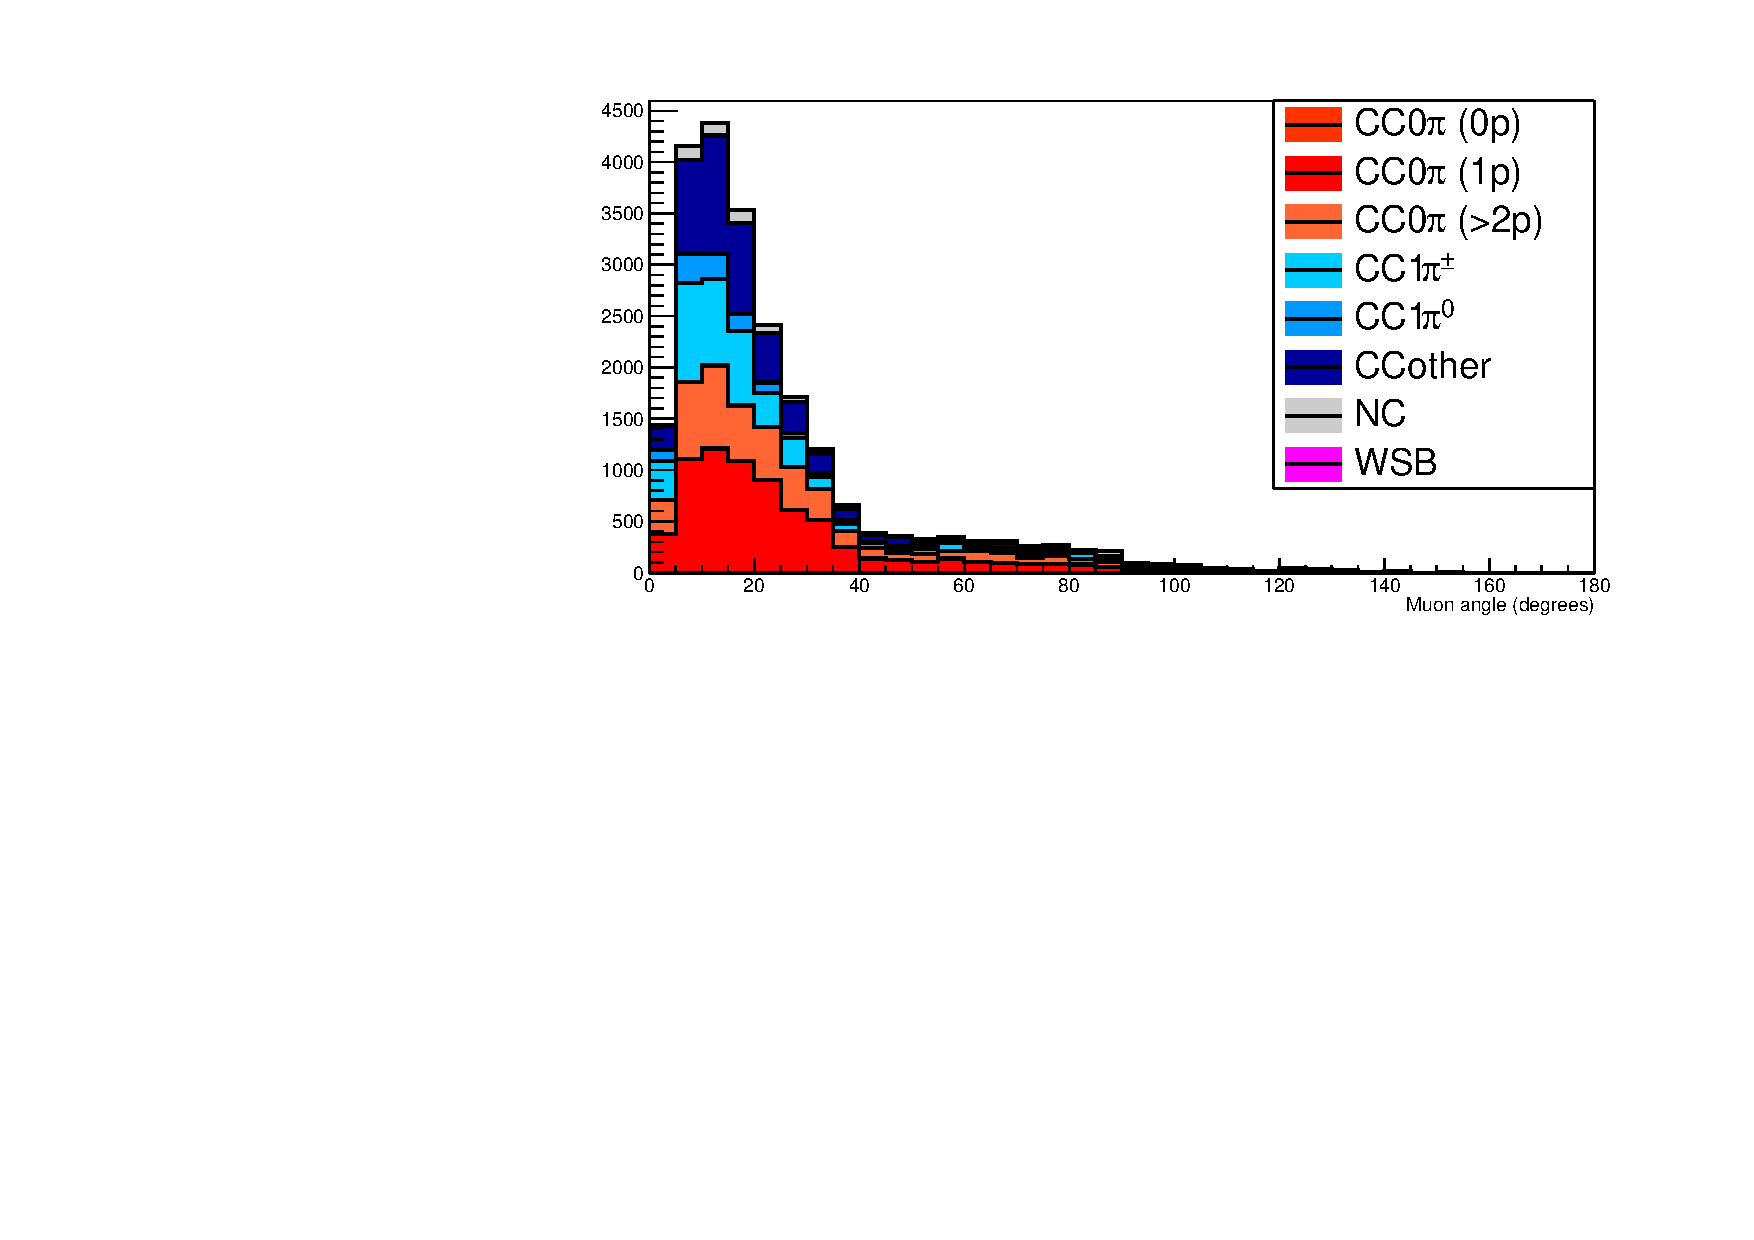
\includegraphics[width=0.55\linewidth, angle=270]{fig/FHCMuonAngle_StoppedOrThroughGoing.pdf}
%     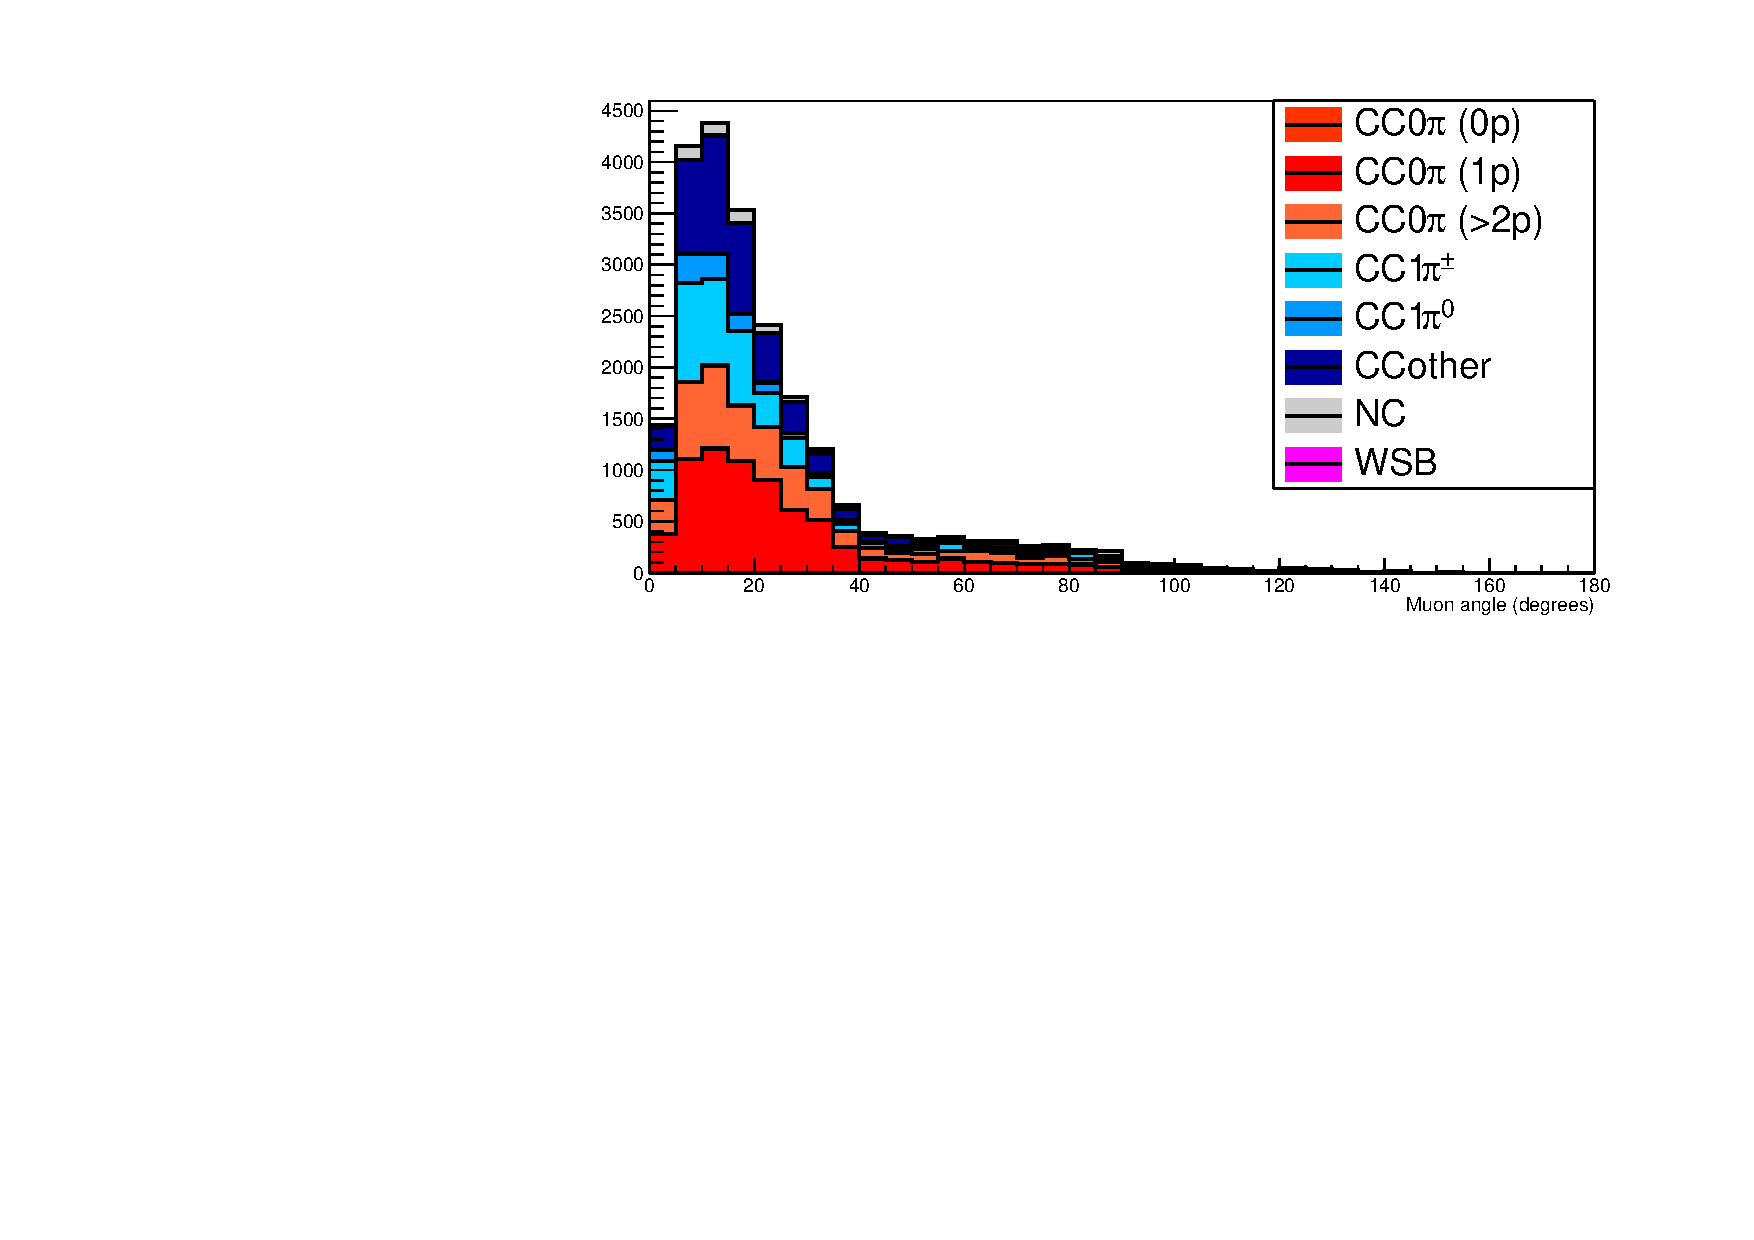
\includegraphics[width=\textwidth]{fig/FHCMuonAngle_StoppedOrThroughGoing.pdf}
    \end{subfigure}
  \begin{subfigure}{0.48\textwidth}
    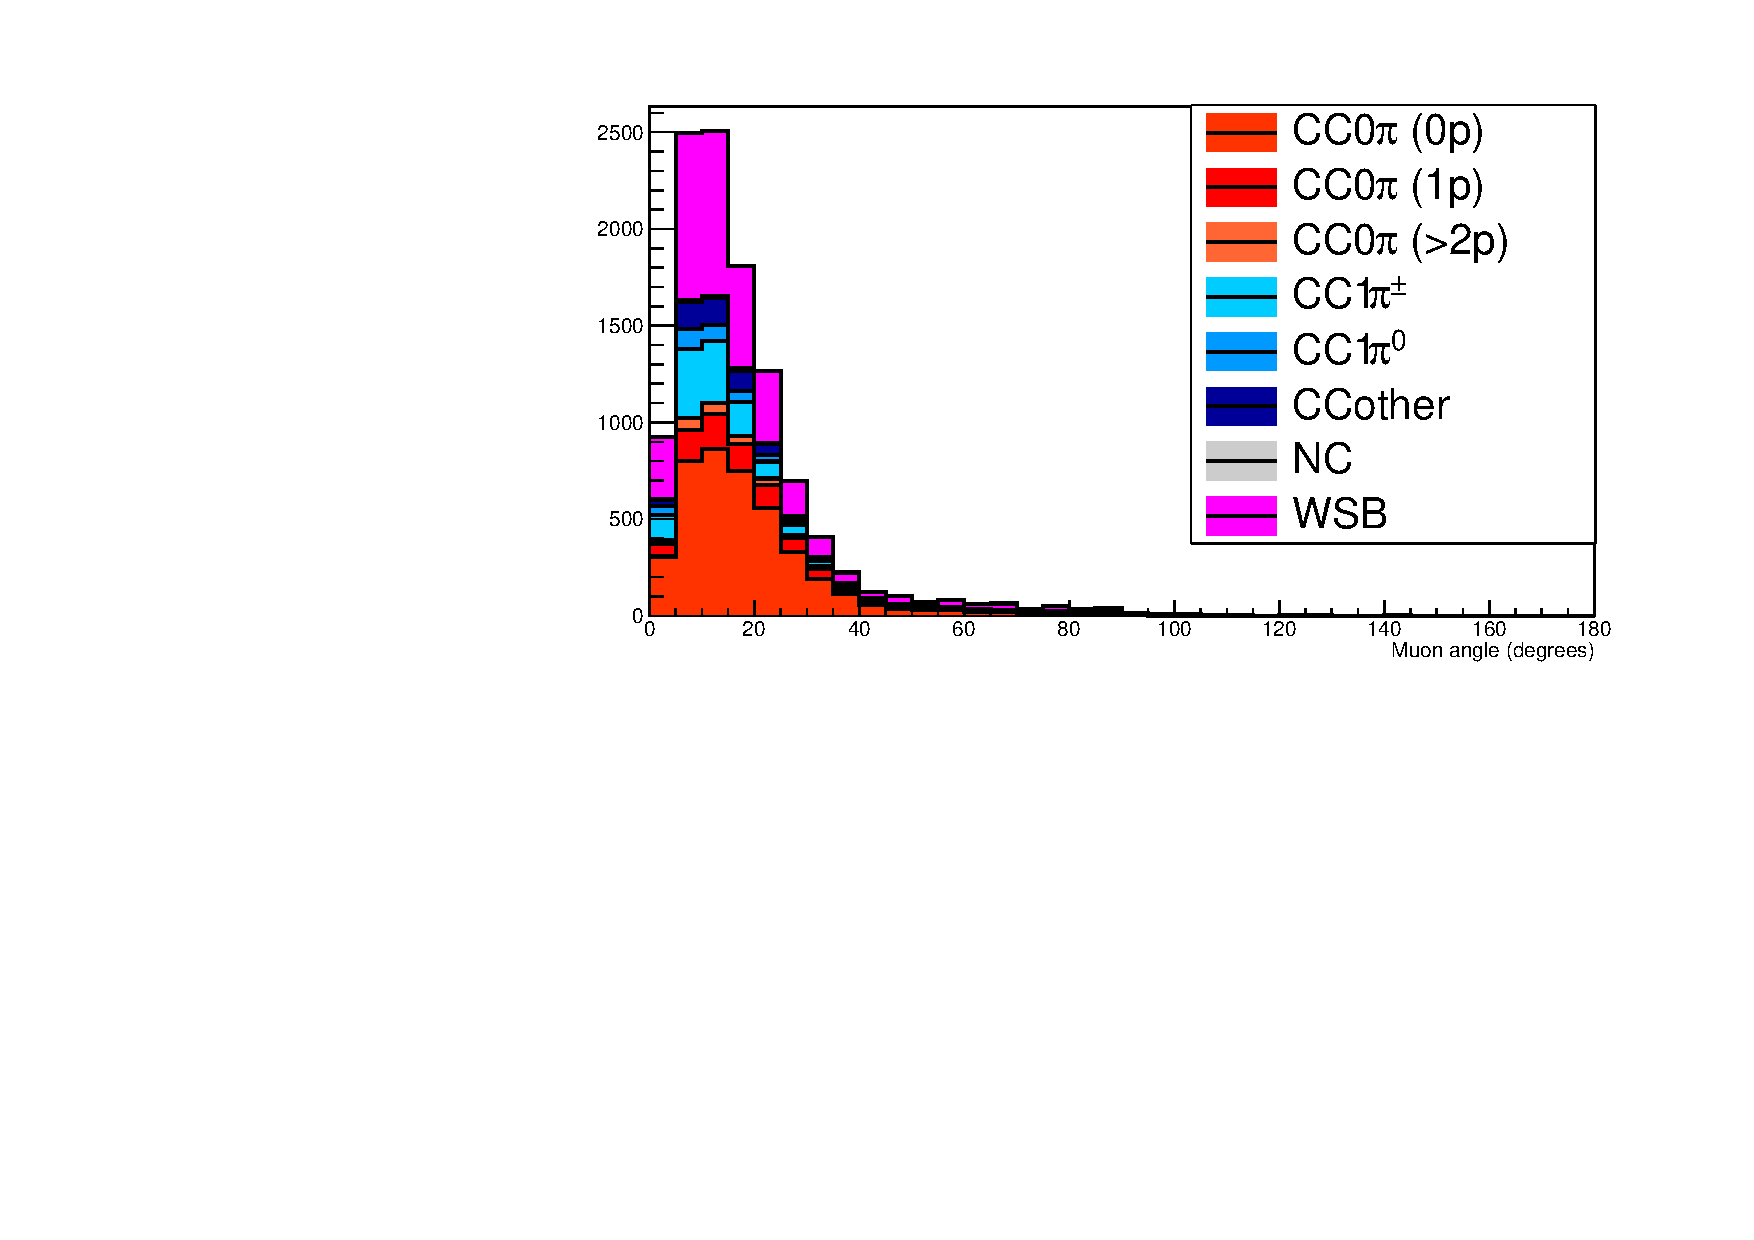
\includegraphics[width=0.55\linewidth, angle=270]{fig/RHCMuonAngle_StoppedOrThroughGoing.pdf}
%    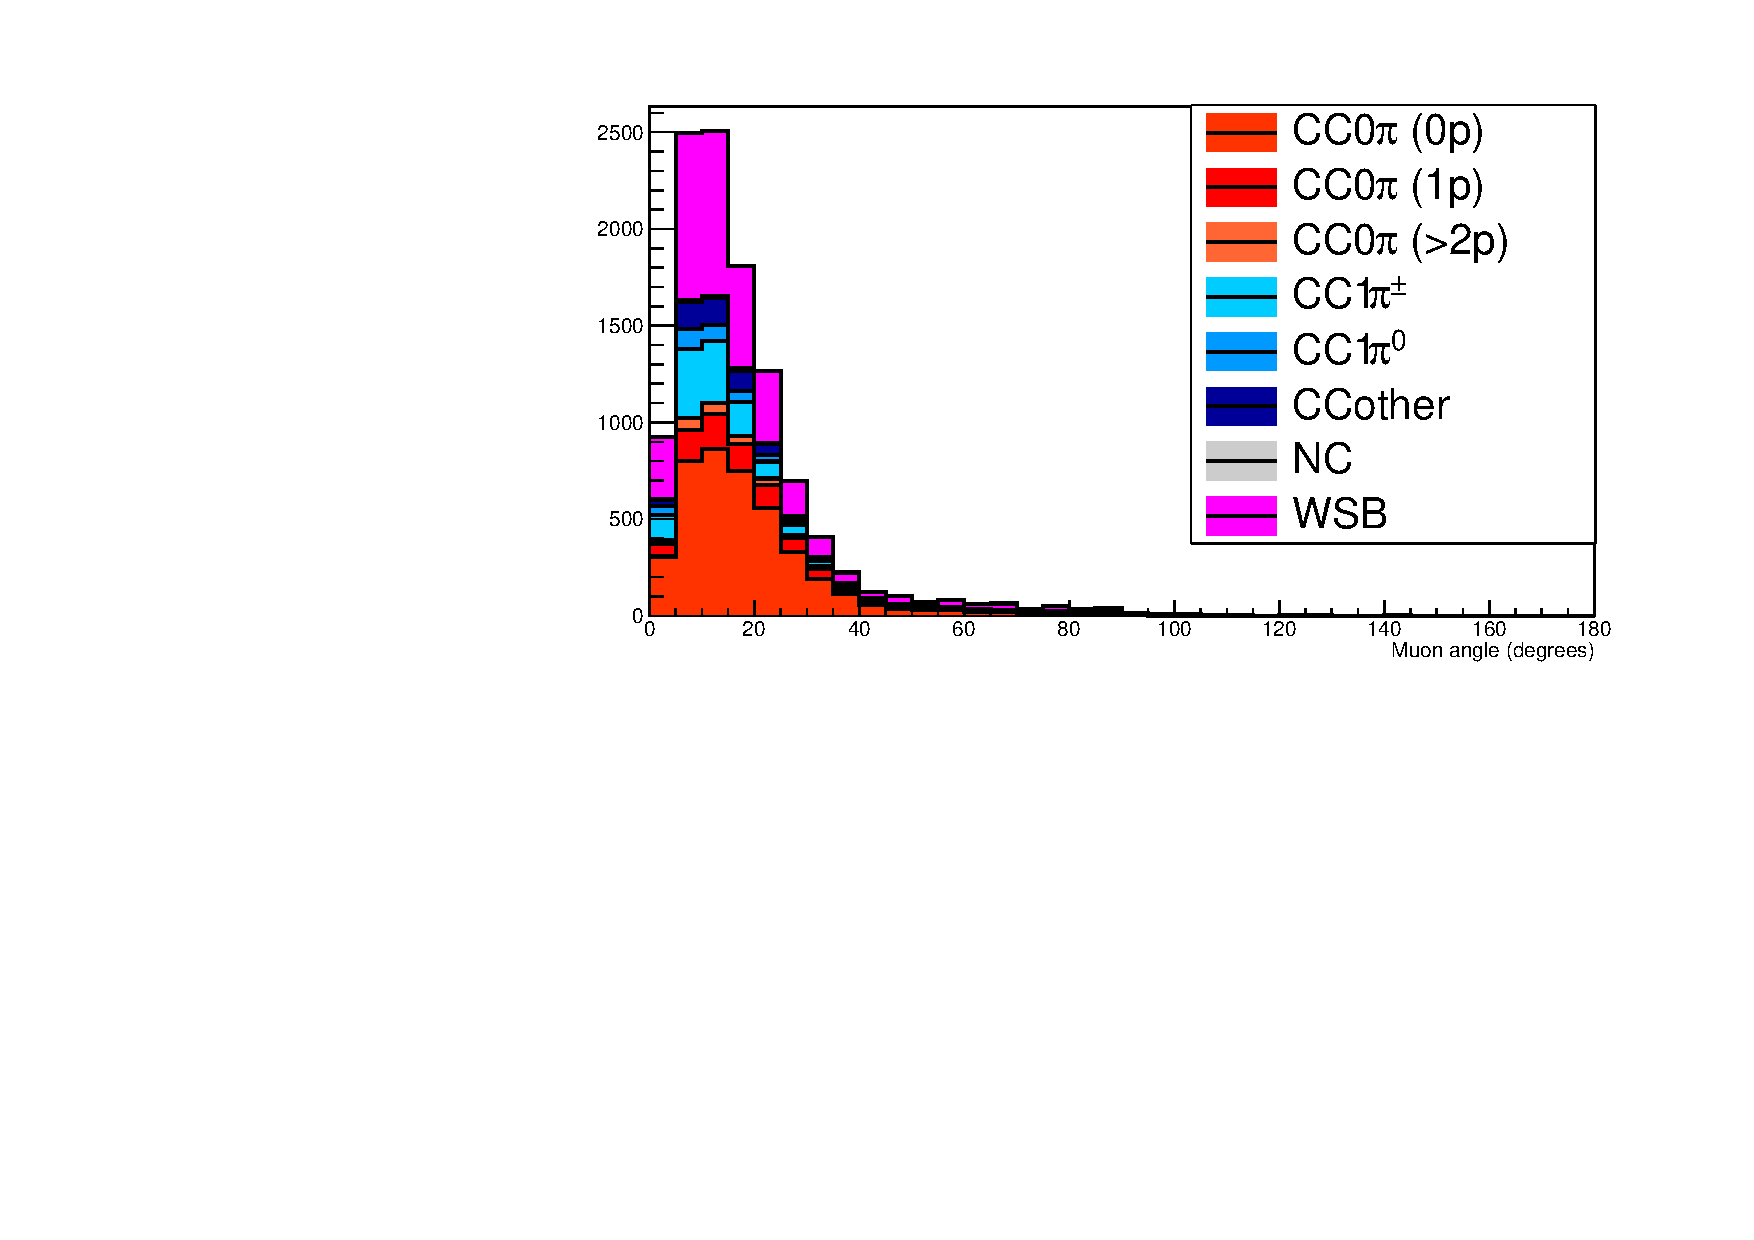
\includegraphics[width=\textwidth]{fig/RHCMuonAngle_StoppedOrThroughGoing.pdf}
    \end{subfigure}    
    \end{center}
  \caption{
The reconstructed angles of the longest tracks in the selected events in the neutrino-mode (left) and the antineutrino-mode (right).
}
\label{fig:angle_allcut}
\end{figure}
%
\begin{figure}[tbh]
 \begin{center}
  \begin{subfigure}{0.48\textwidth}
%     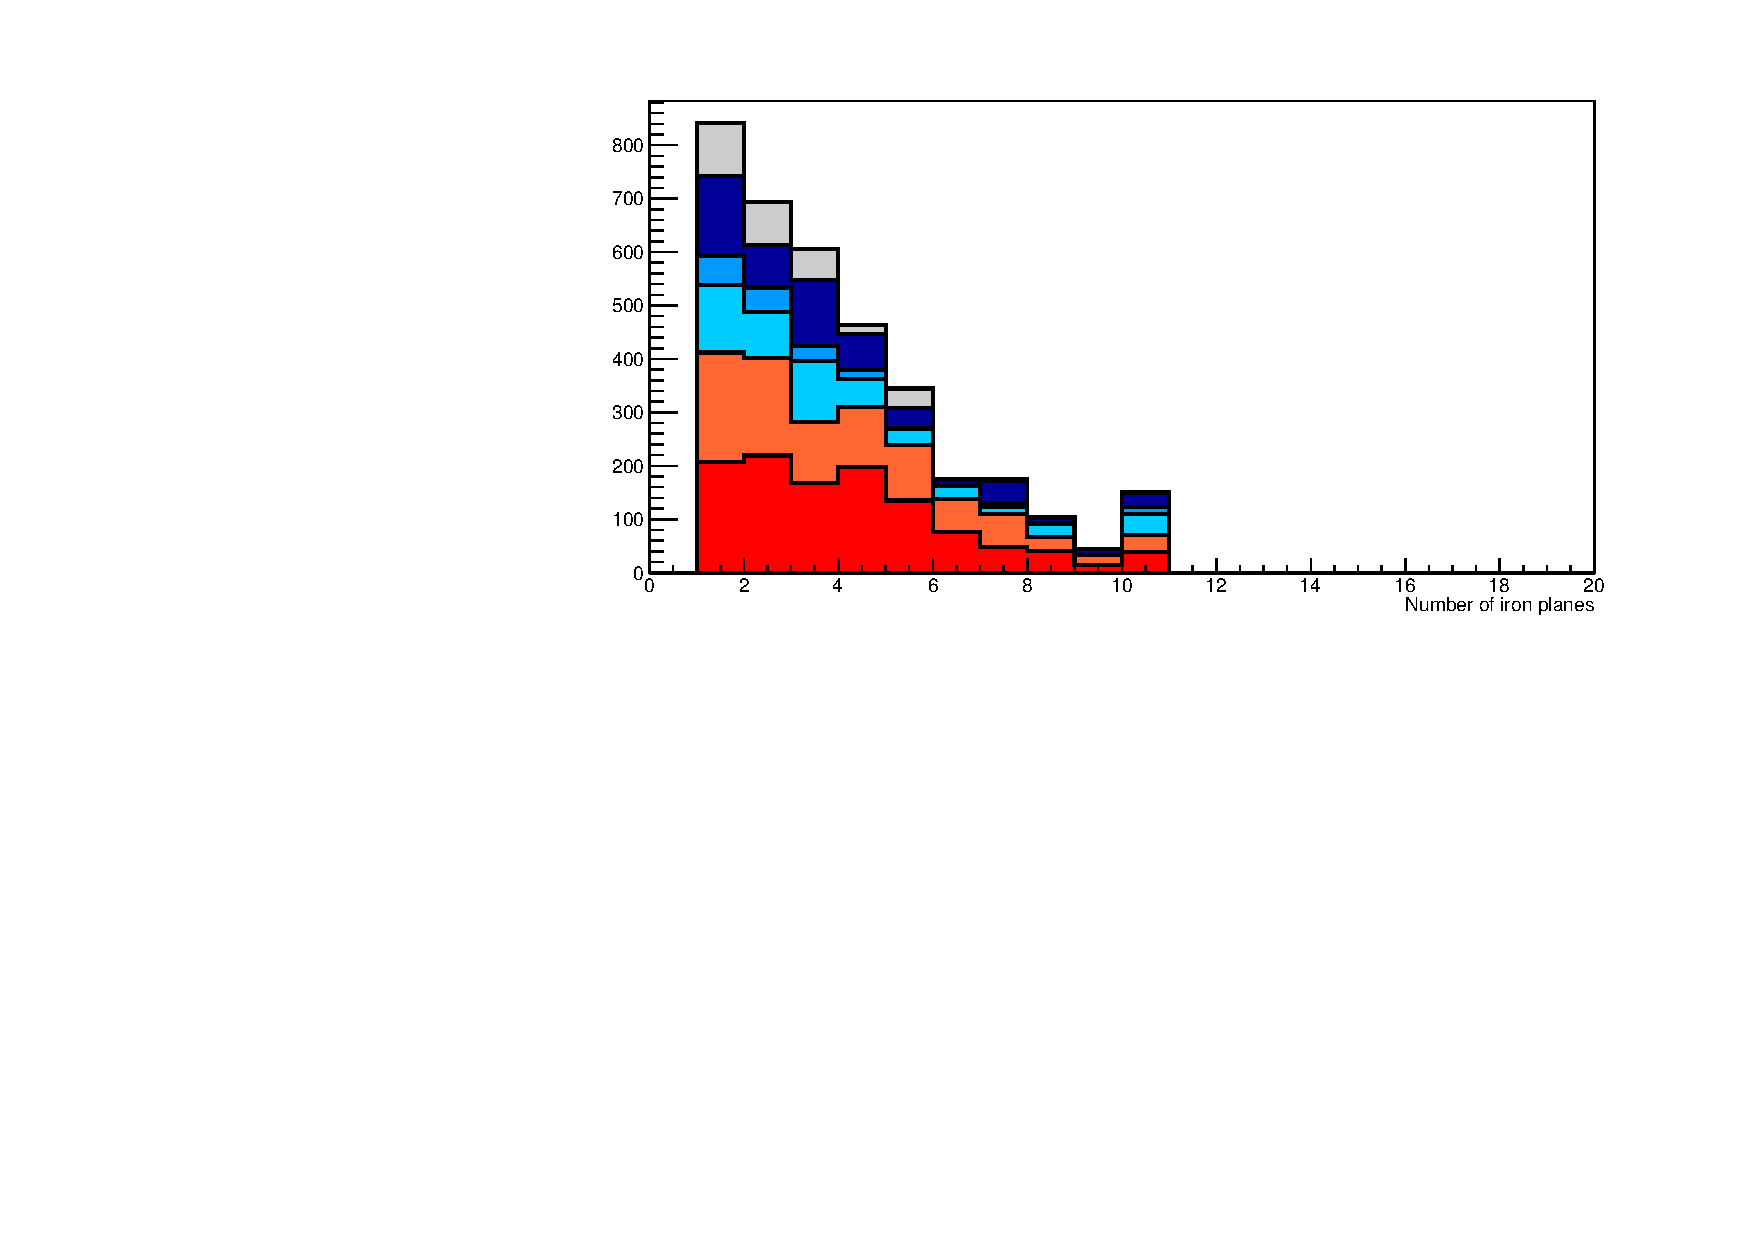
\includegraphics[width=\linewidth]{fig/FHCMuonPenetration_SideMRD_StoppedOrThroughGoing.pdf}
     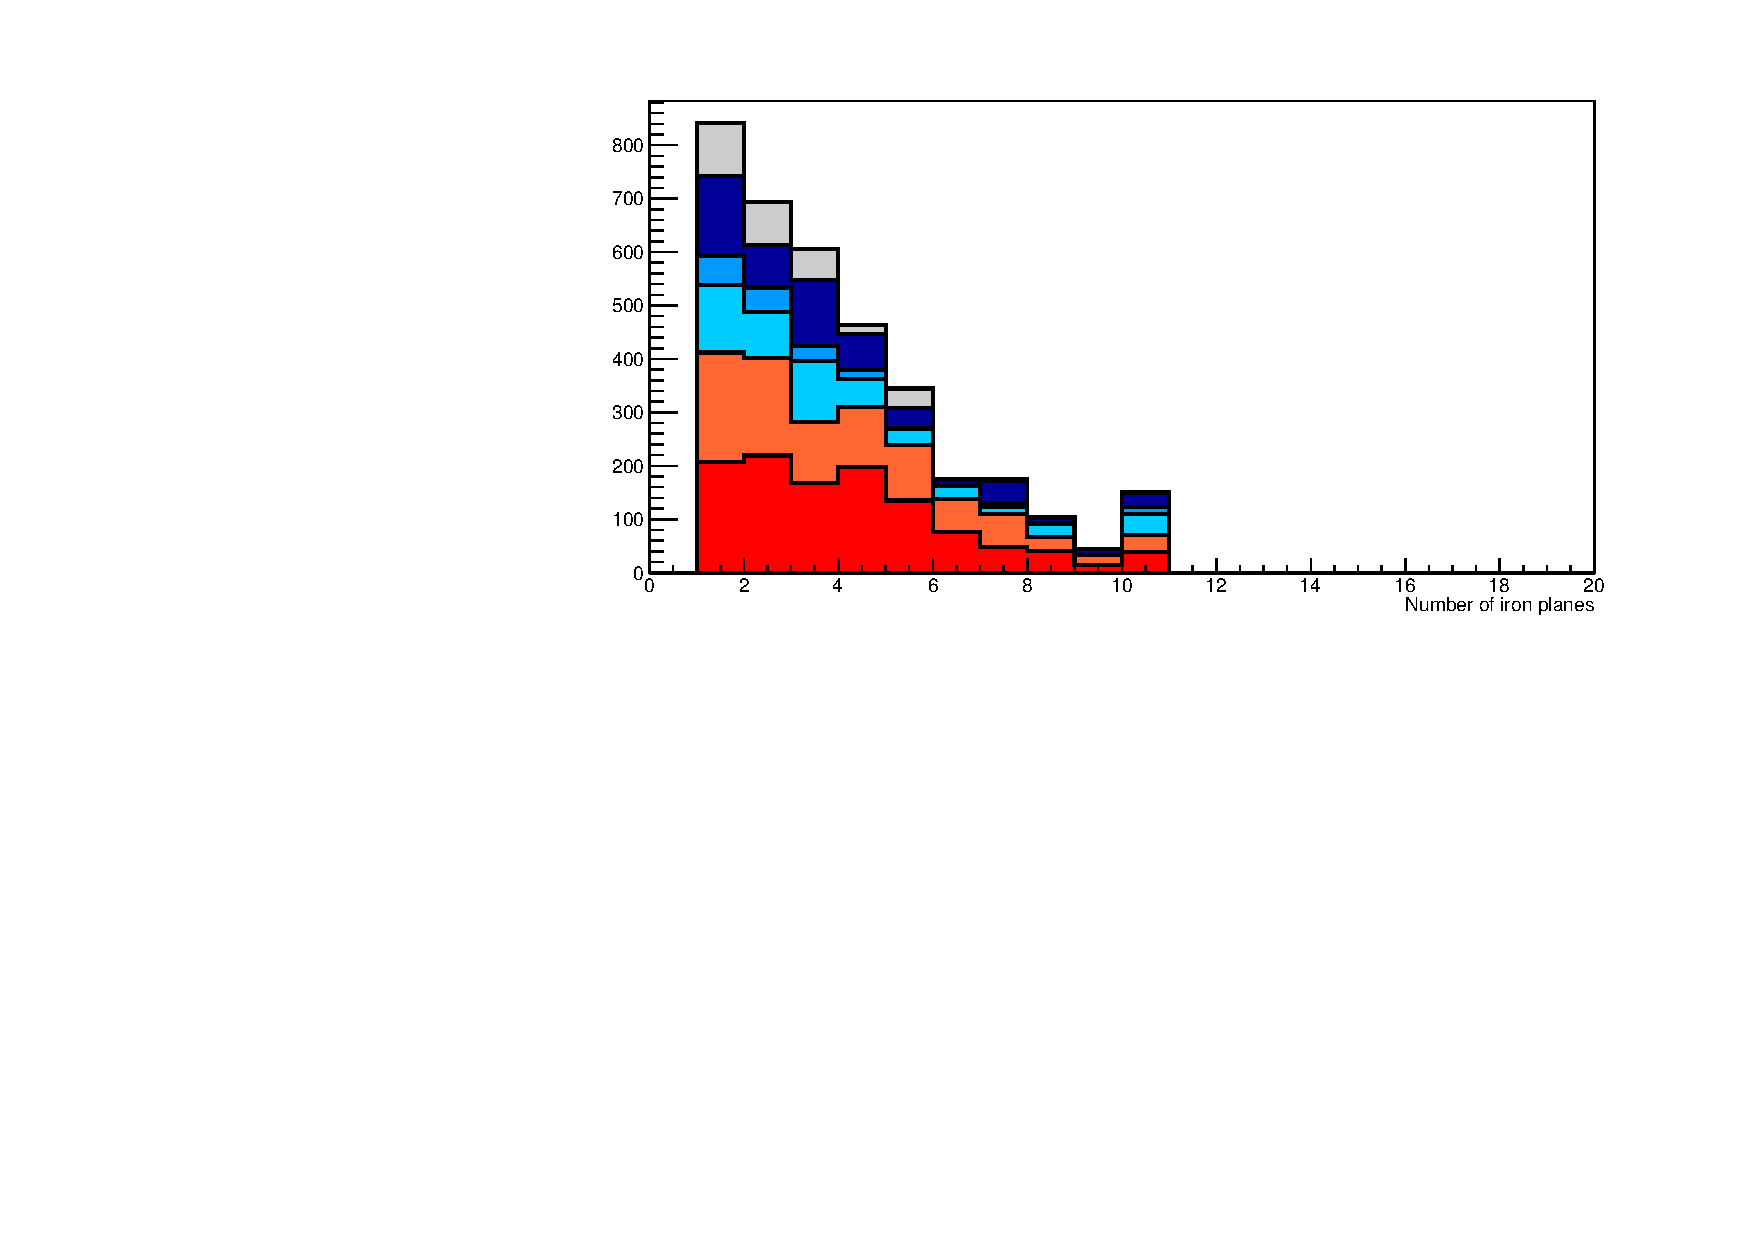
\includegraphics[width=0.55\linewidth, angle=270]{fig/FHCMuonPenetration_SideMRD_StoppedOrThroughGoing.pdf}
    \end{subfigure}
  \begin{subfigure}{0.48\textwidth}
%    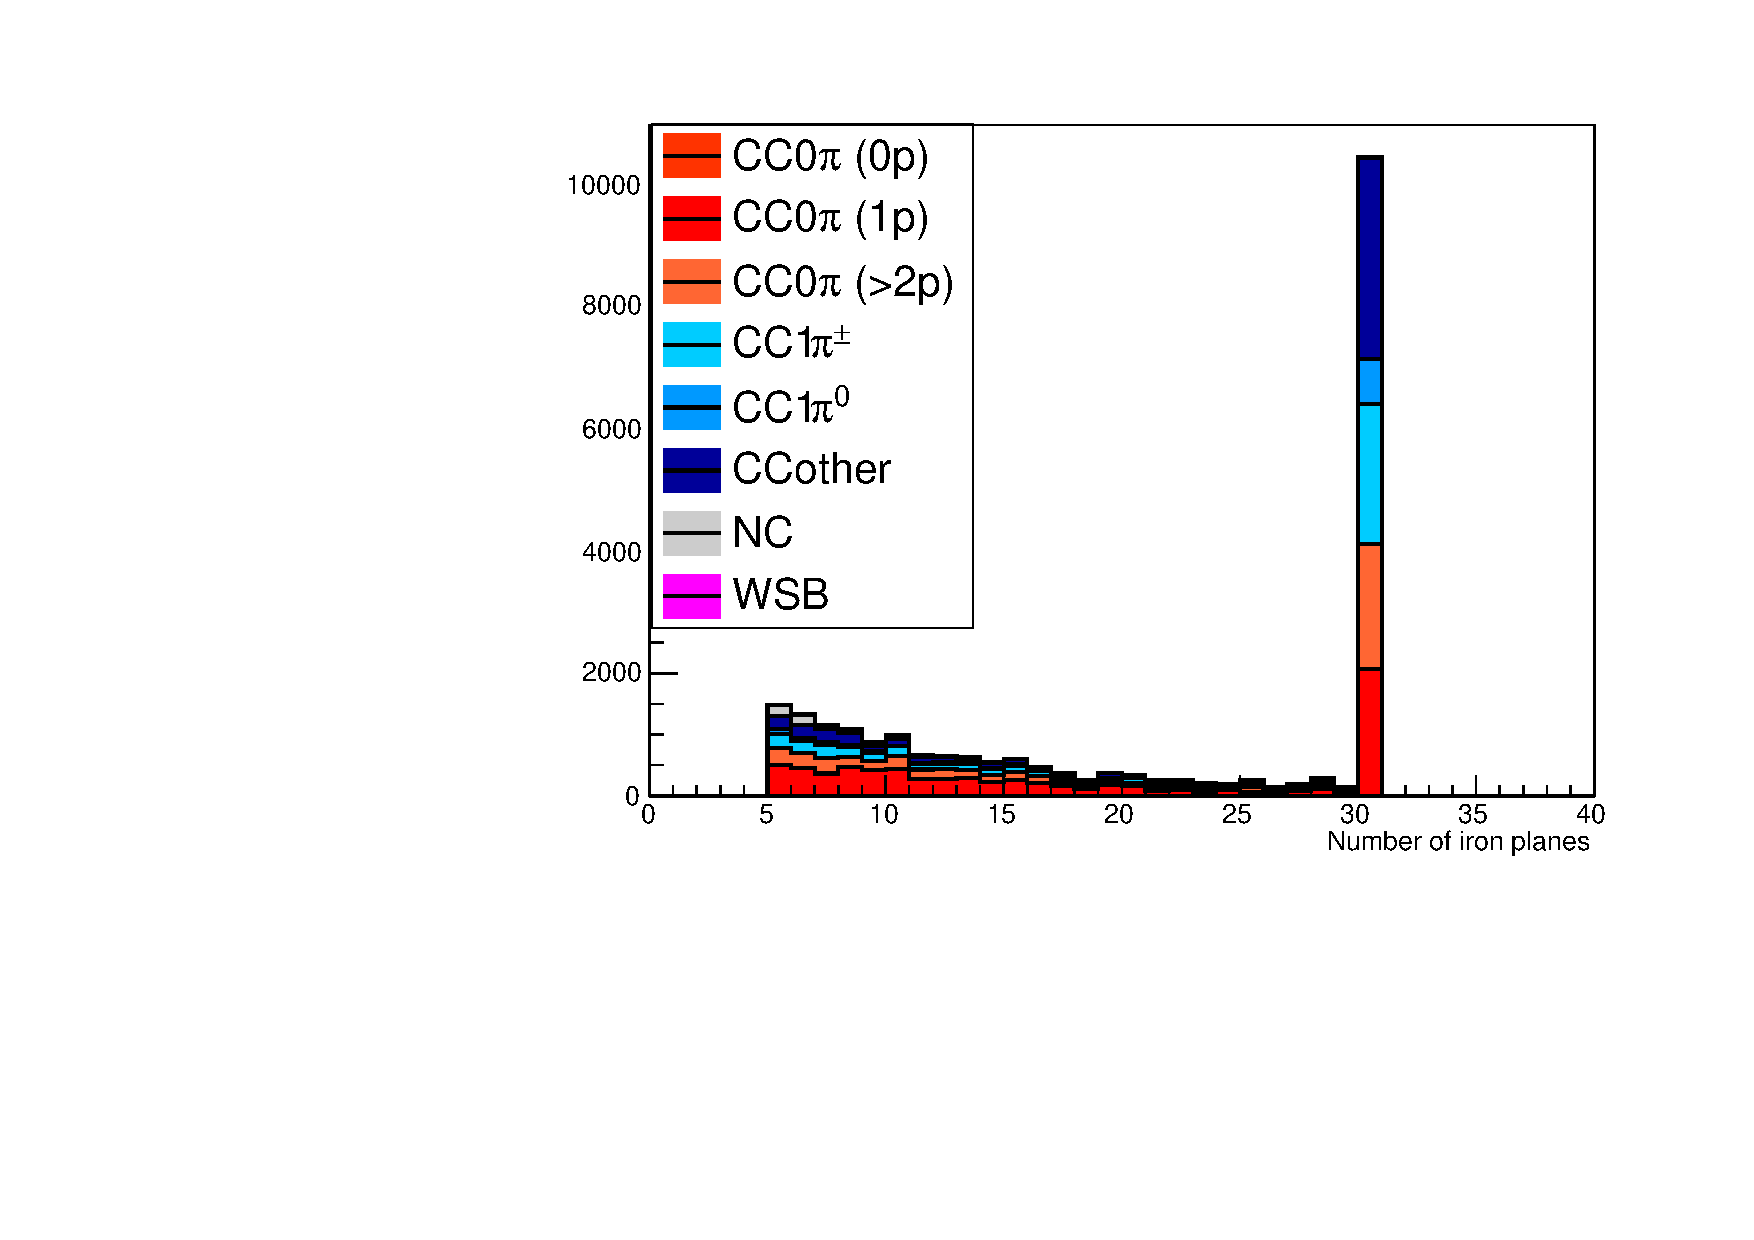
\includegraphics[width=\linewidth]{fig/FHCMuonPenetration_DownstreamMRD_StoppedOrThroughGoing.pdf}
    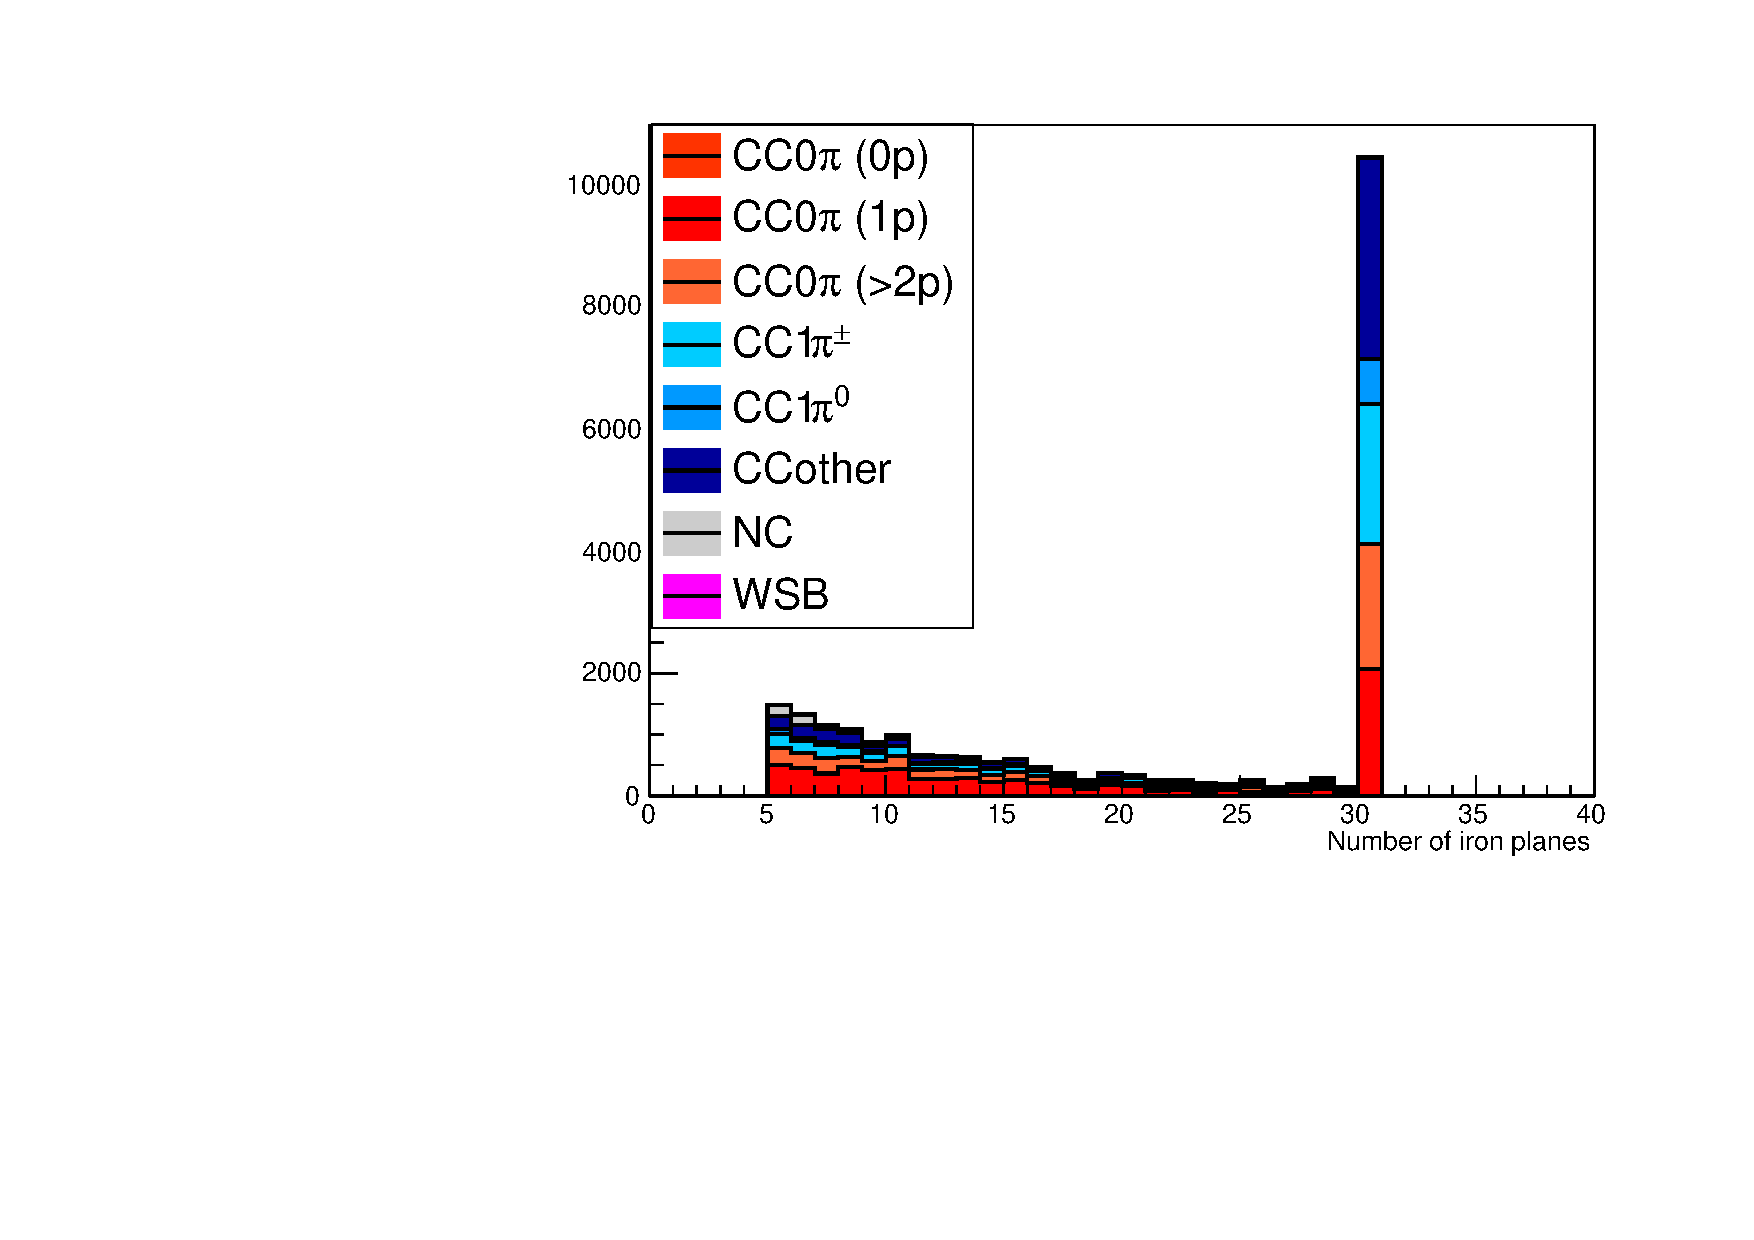
\includegraphics[width=0.55\linewidth, angle=270]{fig/FHCMuonPenetration_DownstreamMRD_StoppedOrThroughGoing.pdf}
    \end{subfigure}  
     \begin{subfigure}{0.48\textwidth}
%     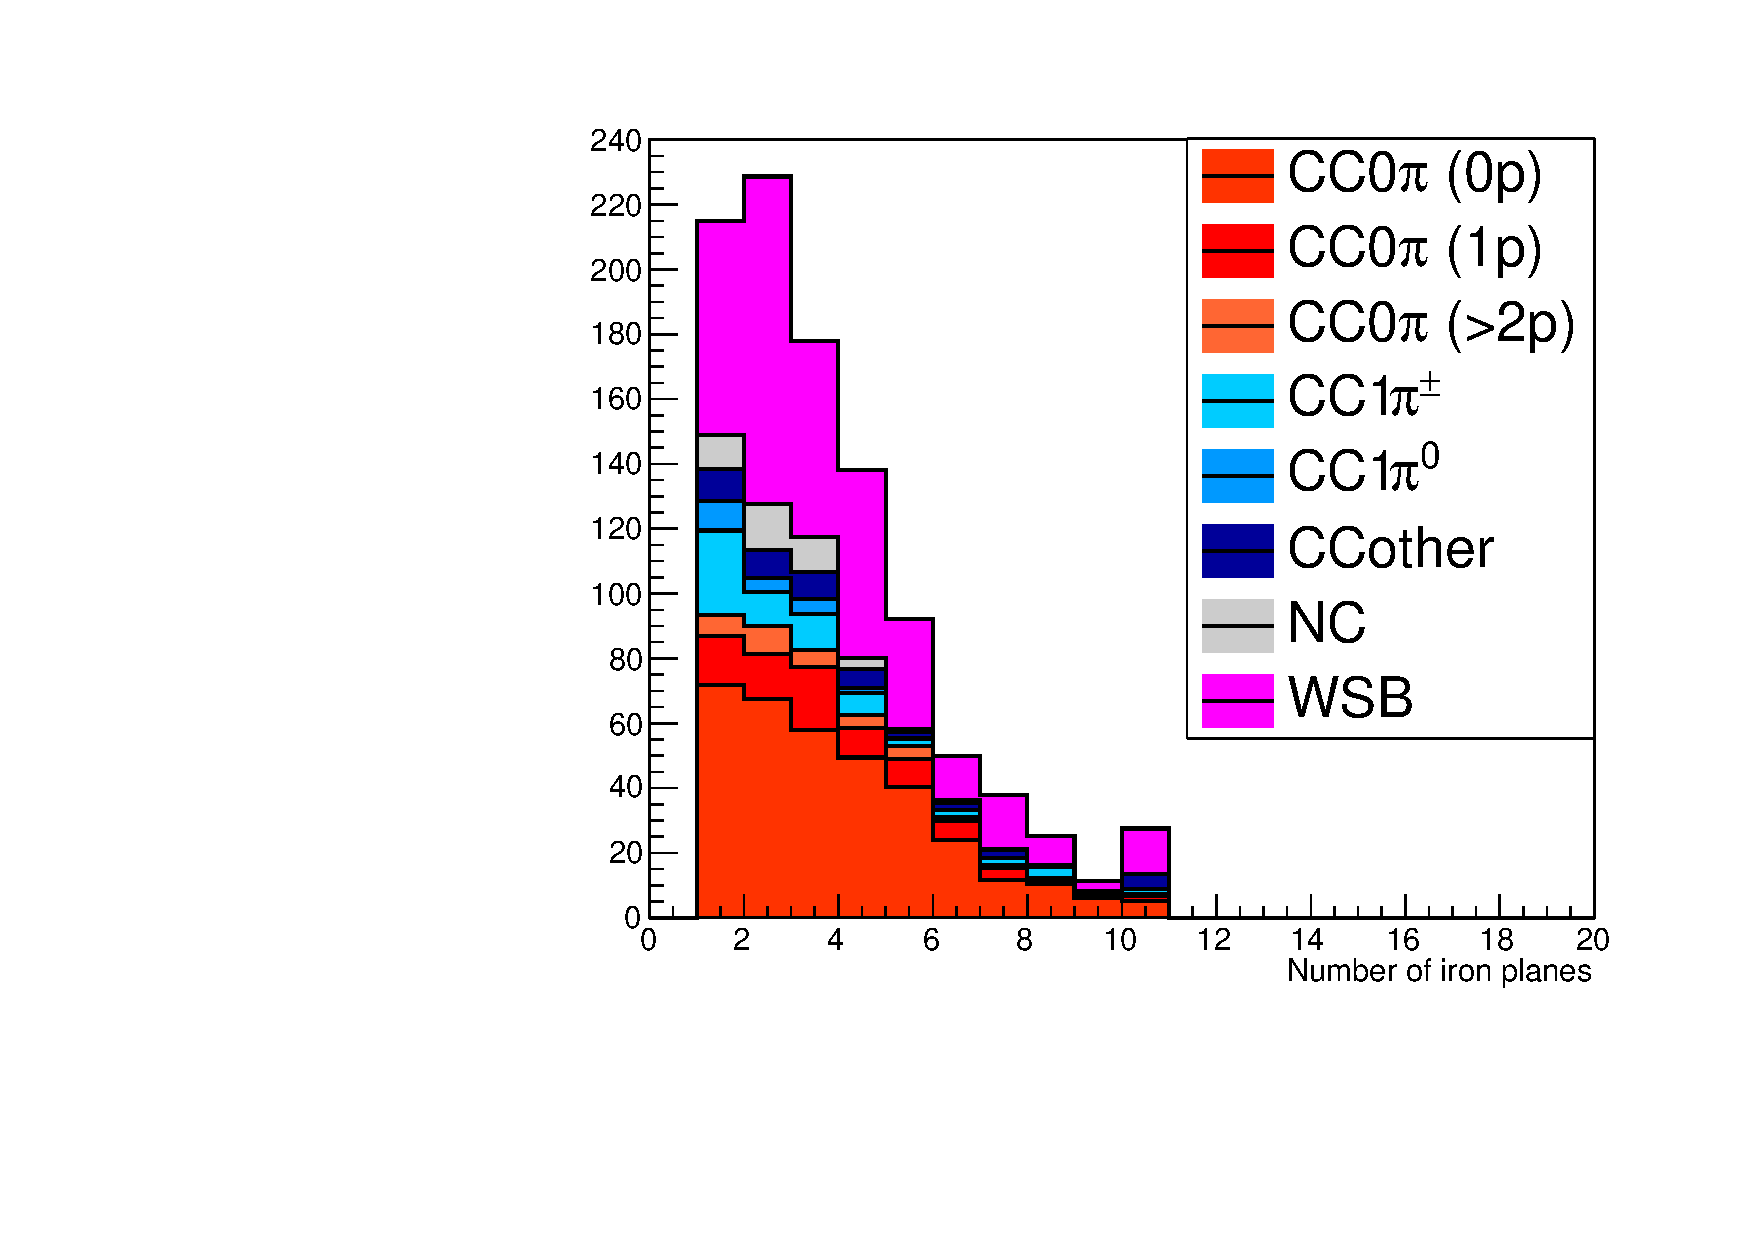
\includegraphics[width=\linewidth]{fig/RHCMuonPenetration_SideMRD_StoppedOrThroughGoing.pdf}
     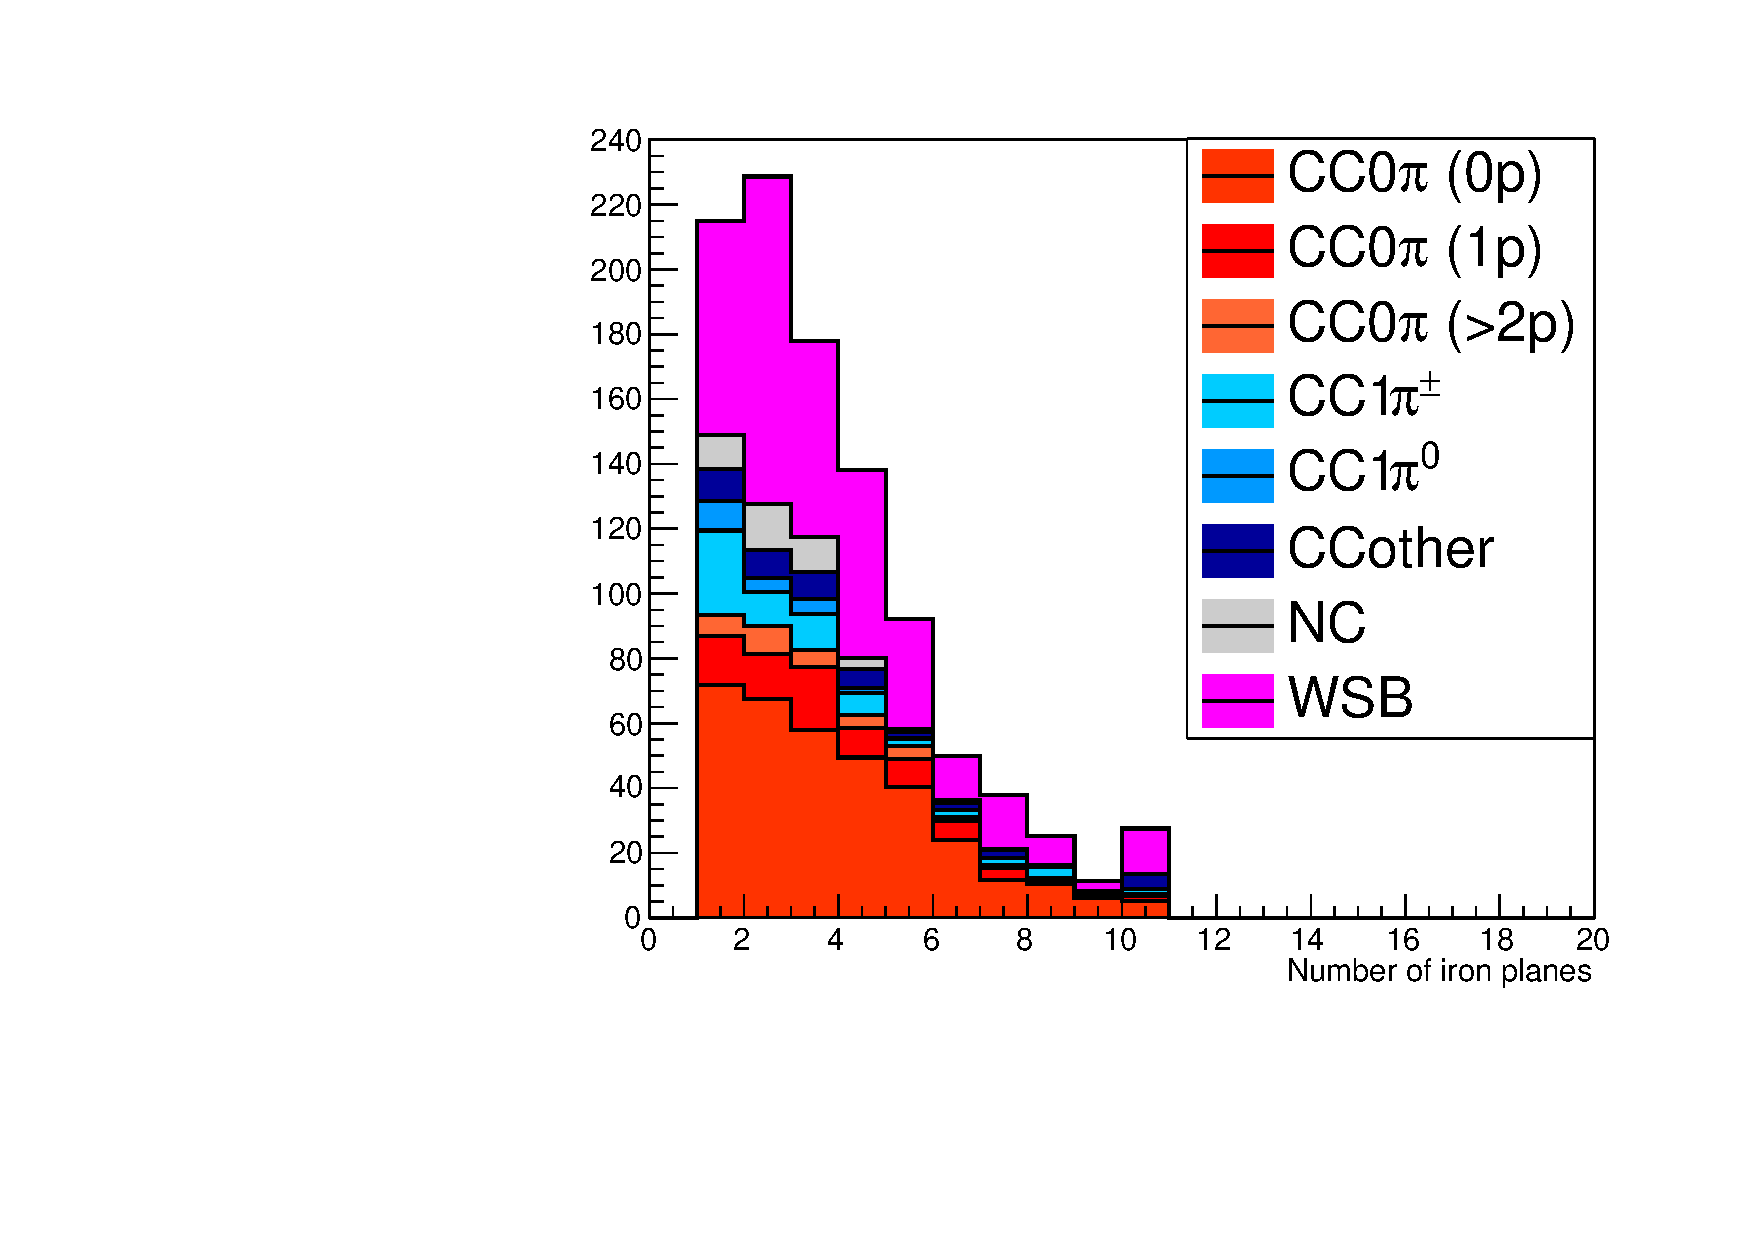
\includegraphics[width=0.55\linewidth, angle=270]{fig/RHCMuonPenetration_SideMRD_StoppedOrThroughGoing.pdf}
    \end{subfigure}
  \begin{subfigure}{0.48\textwidth}
%    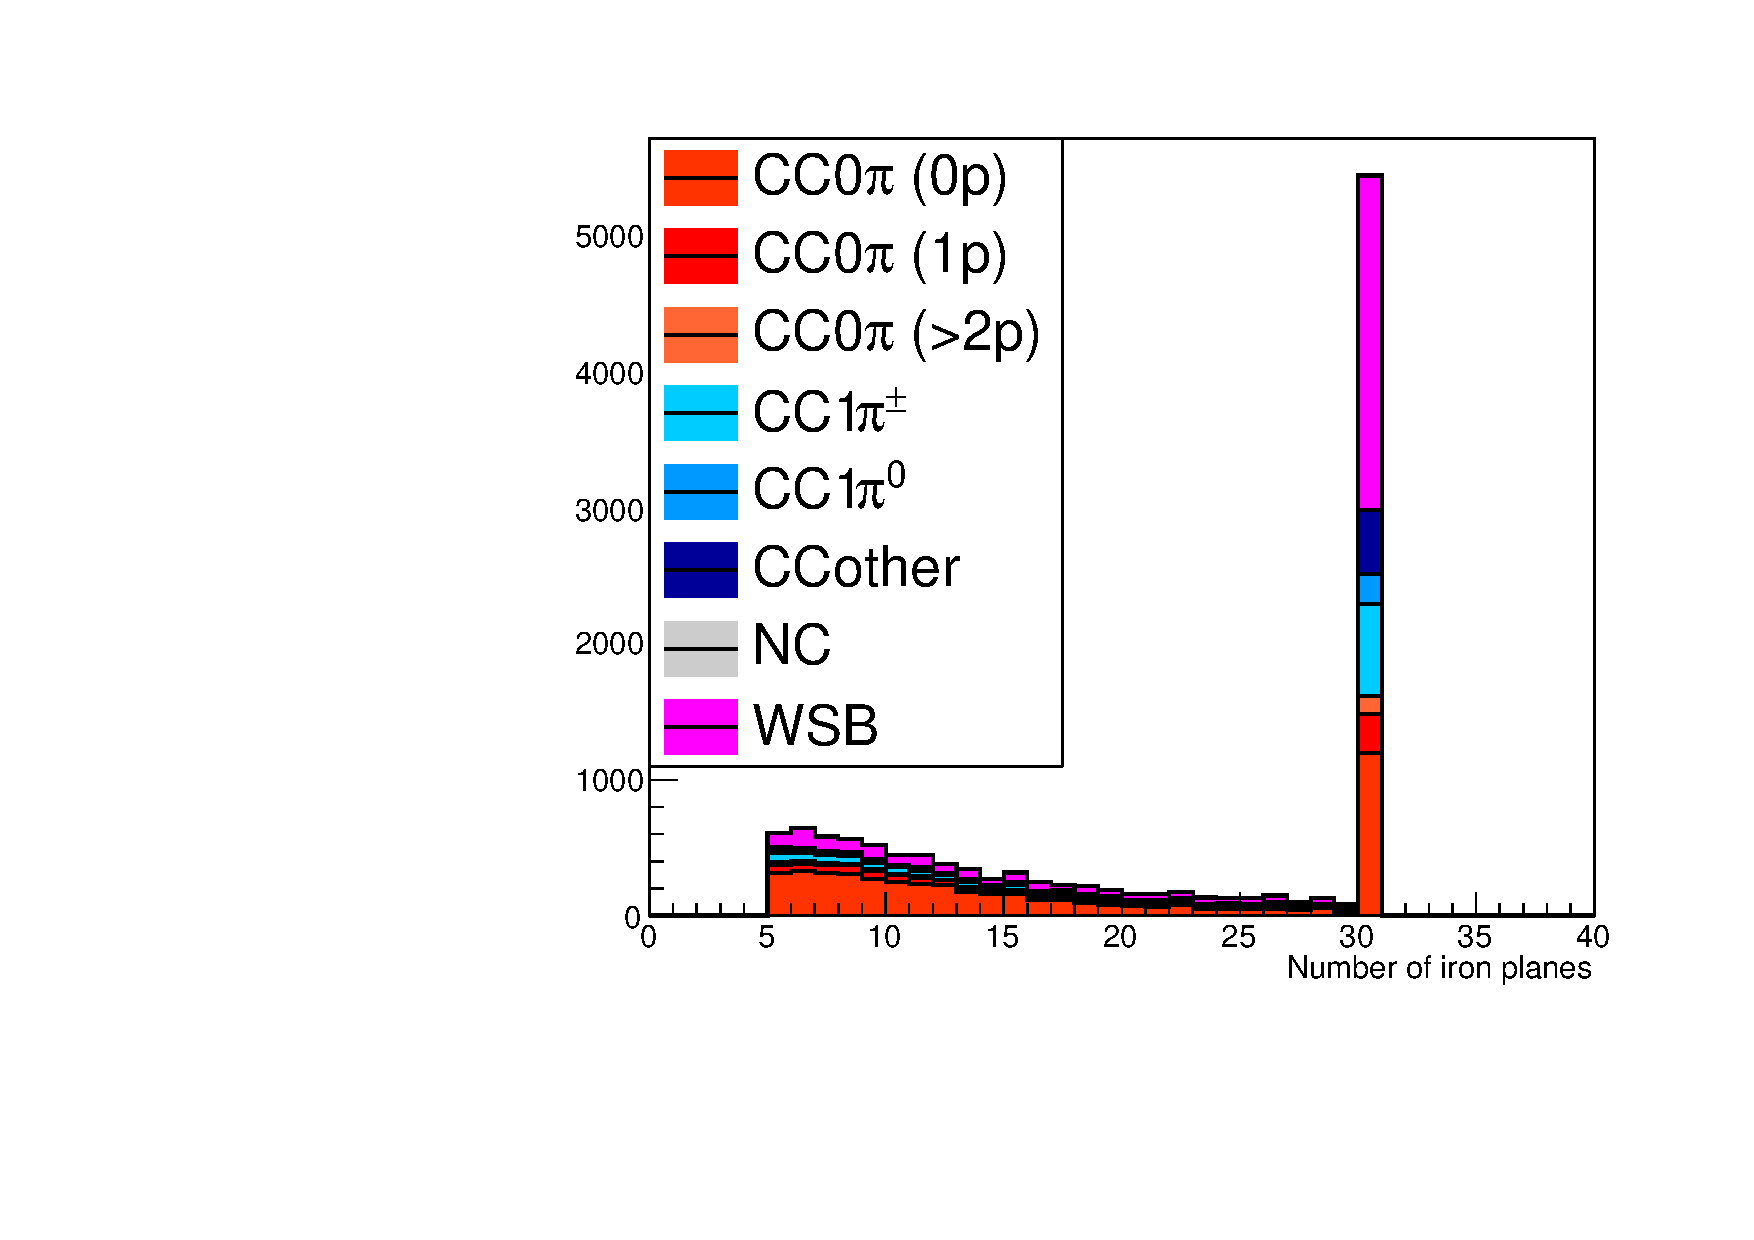
\includegraphics[width=\linewidth]{fig/RHCMuonPenetration_DownstreamMRD_StoppedOrThroughGoing.pdf}
    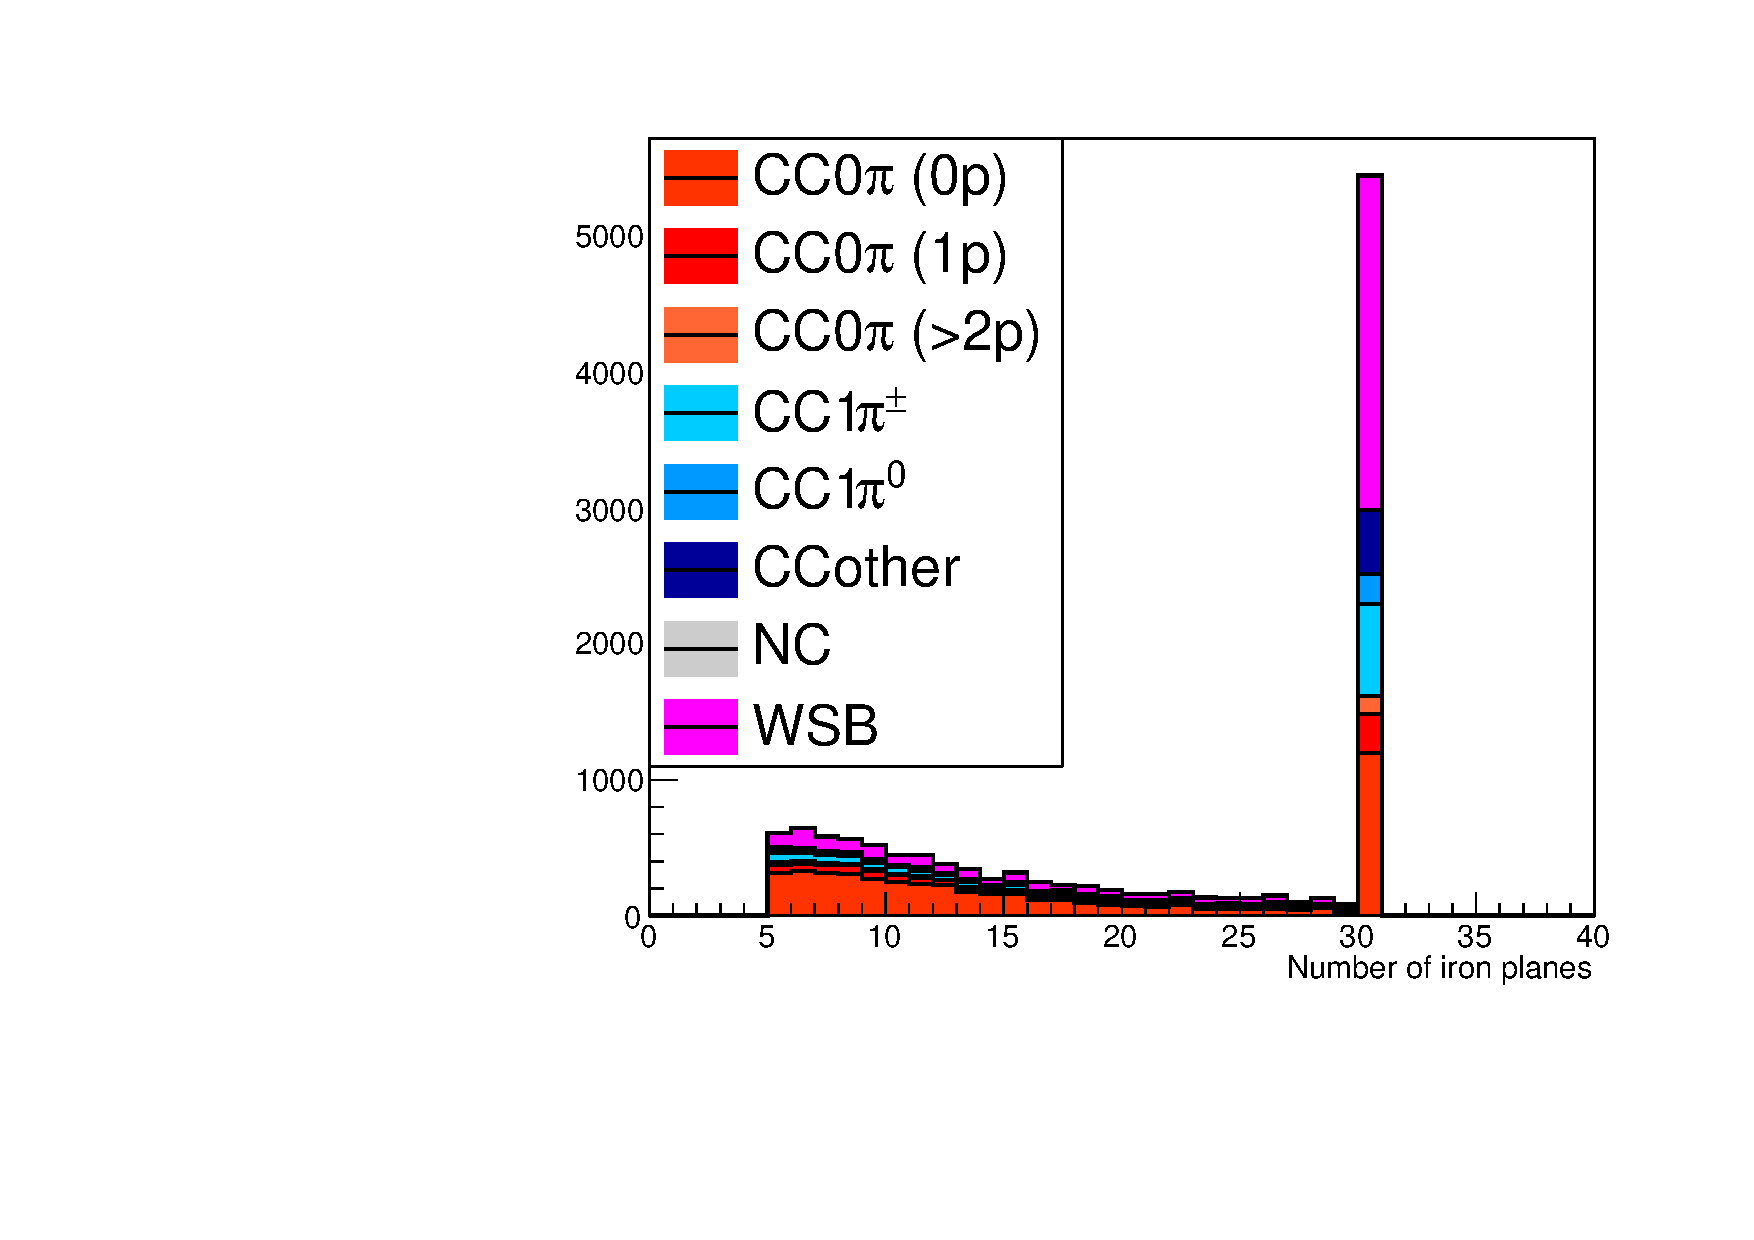
\includegraphics[width=0.55\linewidth, angle=270]{fig/RHCMuonPenetration_DownstreamMRD_StoppedOrThroughGoing.pdf}
    \end{subfigure}    
    \end{center}
  \caption{
Iron plane numbers in Side-MRD (left) and Baby-MIND (right) corresponding to the end points of the longest tracks in the selected events in the neutrino-mode (top) and the antineutrino-mode (bottom).
}
\label{fig:fig:endpoint_longest_track}
\end{figure}



%Table \ref{tab:longest_track_particle} shows particles which produce the longest tracks in the selected events, and the fraction of muons is 85.6\%.
%
%\begin{table}[htb]
% \begin{center}
%   \caption{Particles which produce the longest tracks in the selected events.}
 %   \begin{tabular}{cc} \hline
 %     particles & fraction \\ \hline
 %     $\mu$ & 85.6\% \\
 %     $\pi^{+},\ \pi^{-}$ & 4.8\% \\
 %     p & 4.3\% \\
 %     e$^{+}$, e$^{-}$ & 4.5\% \\
 %     \hline
 %   \end{tabular}
 %   \label{tab:longest_track_particle}
 % \end{center}
% \end{table}

% Figure \ref{fig:eff_muon_angle_momentum_neutrino} shows detection efficiencies of muon tracks in the selected events as a function of muon's true angle and true momentum.
% The efficiency in the large angle region is low because Side-MRD modules only cover sides of the WAGASCI modules.
% The efficiency in the low momentum region is also low because more than two hits  are required to reconstruct the track in the WAGASCI detector.

% \begin{figure}[tbh]
%  \begin{center}
%   \begin{subfigure}{0.48\textwidth}
%     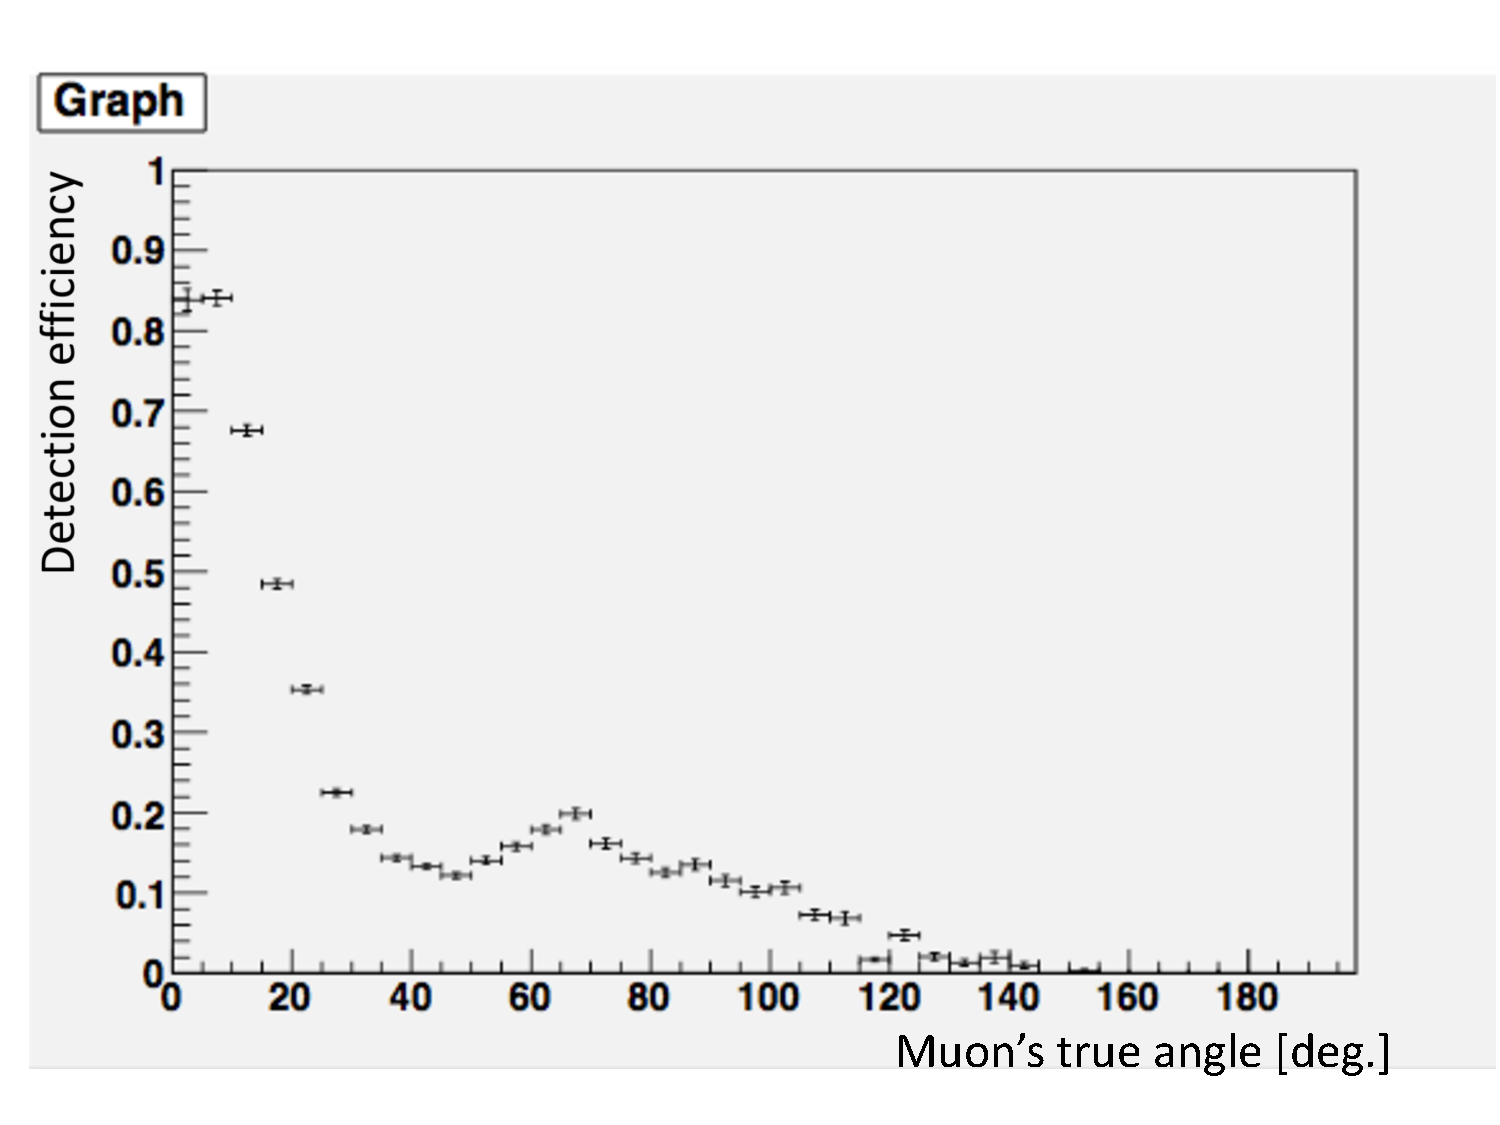
\includegraphics[width=\linewidth]{fig/eff_muon_angle_neutrino.pdf}
%    \end{subfigure}
%  \begin{subfigure}{0.48\textwidth}
%      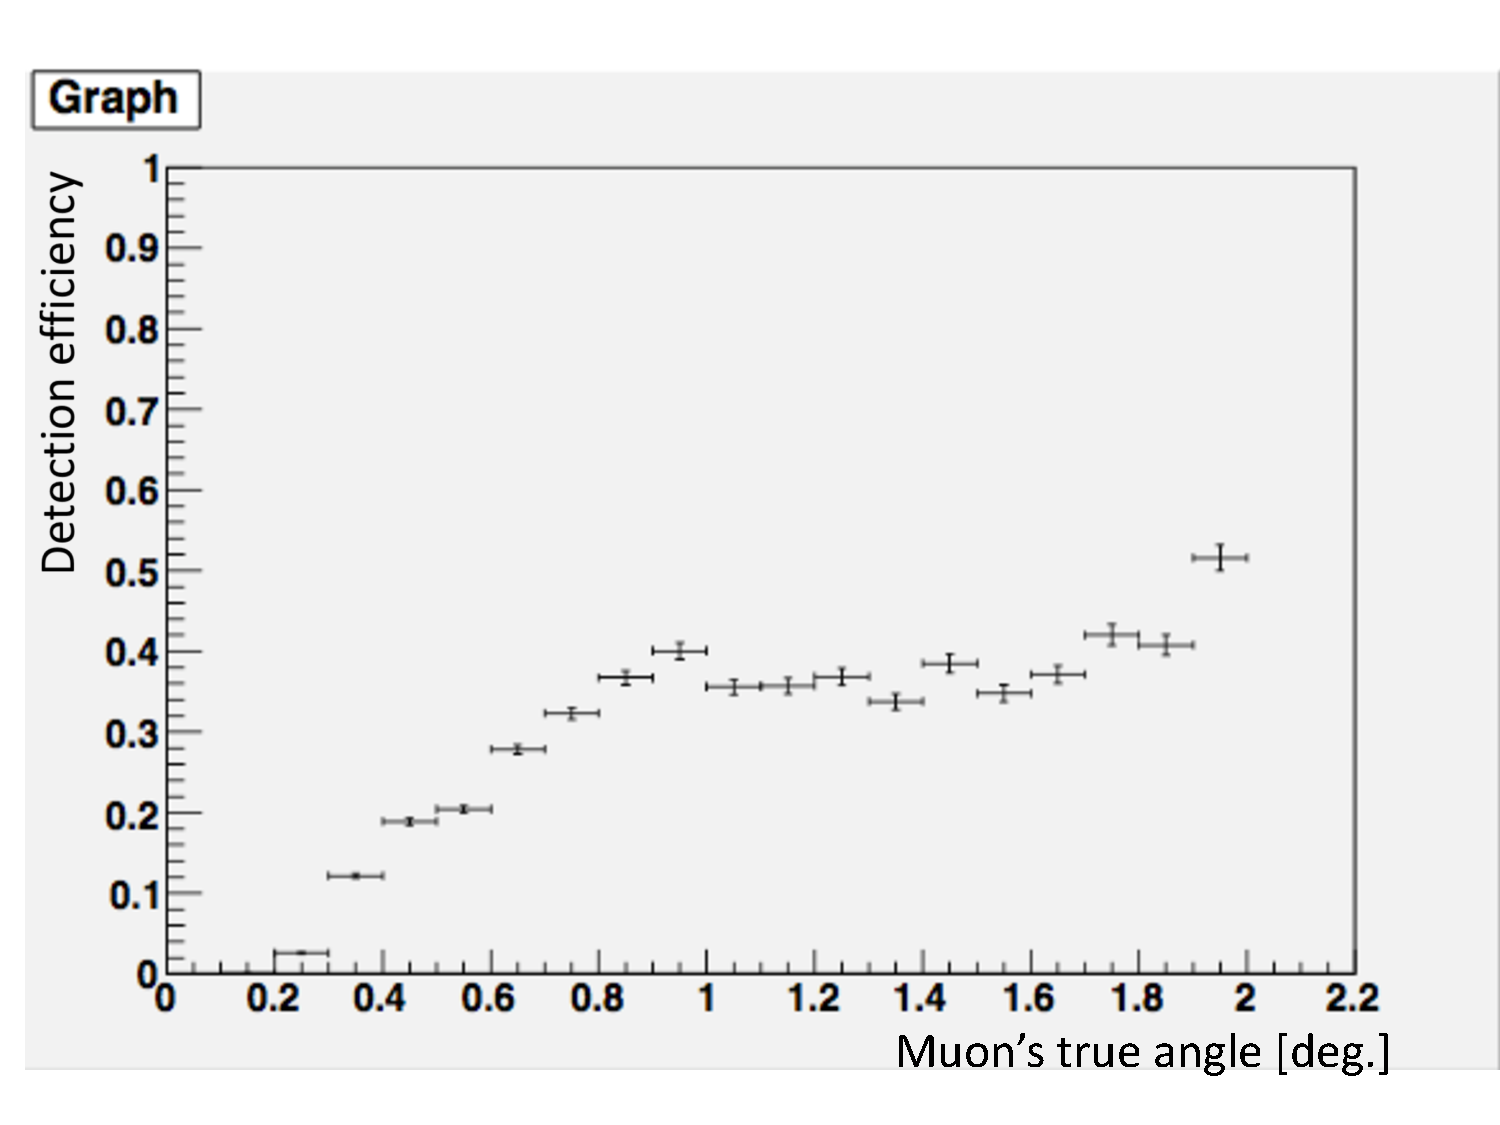
\includegraphics[width=\linewidth]{fig/eff_muon_momentum_neutrino.pdf}
%    \end{subfigure}    
%    \end{center}
%  \caption{
%Detection efficiencies of muon tracks in the selected events as a function of muon's true angle (left) and true momentum (right).
%}
%\label{fig:eff_muon_angle_momentum_neutrino}
%\end{figure}


